\documentclass[a4paper, 12pt]{article}

% packages
\usepackage{amssymb}
\usepackage[fleqn]{mathtools}
\usepackage{tikz}
\usepackage{enumerate}
\usepackage{bussproofs}
\usepackage{xcolor}
\usepackage[margin=1.3cm]{geometry}
\usepackage{logicproof}
\usepackage{diagbox}
\usepackage{listings}
\usepackage{graphicx}
\usepackage{lstautogobble}
\usepackage{hyperref}
\usepackage{multirow}
\usepackage{tipa}
\usepackage{pgfplots}
\usepackage{adjustbox}
\usepackage{dsfont}

% tikz libraries
\usetikzlibrary{
    decorations.pathreplacing,
    arrows,
    shapes,
    shapes.gates.logic.US,
    circuits.logic.US,
    calc,
    automata,
    positioning,
    intersections
}

\pgfplotsset{compat=1.16}

\pgfmathdeclarefunction{gauss}{2}{%
  \pgfmathparse{1/(#2*sqrt(2*pi))*exp(-((x-#1)^2)/(2*#2^2))}%
}

\allowdisplaybreaks % allow environments to break
\setlength\parindent{0pt} % no indent

% shorthand for verbatim
% this clashes with logicproof, so maybe fix this at some point?
\catcode`~=\active
\def~#1~{\texttt{#1}}

% code listing
\lstdefinestyle{main}{
    numberstyle=\tiny,
    breaklines=true,
    showspaces=false,
    showstringspaces=false,
    tabsize=2,
    numbers=left,
    basicstyle=\ttfamily,
    columns=fixed,
    fontadjust=true,
    basewidth=0.5em,
    autogobble,
    xleftmargin=3.0ex,
    mathescape=true
}
\newcommand{\dollar}{\mbox{\textdollar}} %
\lstset{style=main}

% augmented matrix
\makeatletter
\renewcommand*\env@matrix[1][*\c@MaxMatrixCols c]{%
\hskip -\arraycolsep
\let\@ifnextchar\new@ifnextchar
\array{#1}}
\makeatother

% ceiling / floor
\DeclarePairedDelimiter{\ceil}{\lceil}{\rceil}
\DeclarePairedDelimiter{\floor}{\lfloor}{\rfloor}

% custom commands
\newcommand{\indefint}[2]{\int #1 \, \mathrm{d}#2}
\newcommand{\defint}[4]{\int_{#1}^{#2} #3 \, \mathrm{d}#4}
\newcommand{\pdif}[2]{\frac{\partial #1}{\partial #2}}
\newcommand{\dif}[2]{\frac{\mathrm{d}#1}{\mathrm{d}#2}}
\newcommand{\limit}[2]{\raisebox{0.5ex}{\scalebox{0.8}{$\displaystyle{\lim_{#1 \to #2}}$}}}
\newcommand{\limitsup}[2]{\raisebox{0.5ex}{\scalebox{0.8}{$\displaystyle{\limsup_{#1 \to #2}}$}}}
\newcommand{\summation}[2]{\sum\limits_{#1}^{#2}}
\newcommand{\product}[2]{\prod\limits_{#1}^{#2}}
\newcommand{\intbracket}[3]{\left[#3\right]_{#1}^{#2}}
\newcommand{\laplace}{\mathcal{L}}
\newcommand{\fourier}{\mathcal{F}}
\newcommand{\mat}[1]{\boldsymbol{#1}}
\renewcommand{\vec}[1]{\boldsymbol{#1}}
\newcommand{\rowt}[1]{\begin{bmatrix}
    #1
\end{bmatrix}^\top}
\DeclareMathOperator*{\argmax}{argmax}
\DeclareMathOperator*{\argmin}{argmin}

\newcommand{\lto}[0]{\leadsto\ }

\newcommand{\ulsmash}[1]{\underline{\smash{#1}}}

\newcommand{\powerset}[0]{\wp}
\renewcommand{\emptyset}[0]{\varnothing}

\makeatletter
\newsavebox{\@brx}
\newcommand{\llangle}[1][]{\savebox{\@brx}{\(\m@th{#1\langle}\)}%
  \mathopen{\copy\@brx\kern-0.5\wd\@brx\usebox{\@brx}}}
\newcommand{\rrangle}[1][]{\savebox{\@brx}{\(\m@th{#1\rangle}\)}%
  \mathclose{\copy\@brx\kern-0.5\wd\@brx\usebox{\@brx}}}
\makeatother
\newcommand{\lla}{\llangle}
\newcommand{\rra}{\rrangle}
\newcommand{\la}{\langle}
\newcommand{\ra}{\rangle}
\newcommand{\crnr}[1]{\text{\textopencorner} #1 \text{\textcorner}}
\newcommand{\bnfsep}[0]{\ |\ }
\newcommand{\concsep}[0]{\ ||\ }

\newcommand{\axiom}[1]{\AxiomC{#1}}
\newcommand{\unary}[1]{\UnaryInfC{#1}}
\newcommand{\binary}[1]{\BinaryInfC{#1}}
\newcommand{\trinary}[1]{\TrinaryInfC{#1}}
\newcommand{\quaternary}[1]{\QuaternaryInfC{#1}}
\newcommand{\quinary}[1]{\QuinaryInfC{#1}}
\newcommand{\dproof}[0]{\DisplayProof}
\newcommand{\llabel}[1]{\LeftLabel{\scriptsize #1}}
\newcommand{\rlabel}[1]{\RightLabel{\scriptsize #1}}

\newcommand{\ttbs}{\char`\\}
\newcommand{\lrbt}[0]{\ \bullet\ }

% colours
\newcommand{\violet}[1]{\textcolor{violet}{#1}}
\newcommand{\blue}[1]{\textcolor{blue}{#1}}
\newcommand{\red}[1]{\textcolor{red}{#1}}
\newcommand{\teal}[1]{\textcolor{teal}{#1}}

% reasoning proofs
\usepackage{ltablex}
\usepackage{environ}
\keepXColumns
\NewEnviron{reasoning}{
    \begin{tabularx}{\textwidth}{rlX}
        \BODY
    \end{tabularx}
}
\newcommand{\proofline}[3]{$(#1)$ & $#2$ & \hfill #3 \smallskip \\}
\newcommand{\proofarbitrary}[1]{& take arbitrary $#1$ \smallskip \\}
\newcommand{\prooftext}[1]{\multicolumn{3}{l}{#1} \smallskip \\}
\newcommand{\proofmath}[3]{$#1$ & = $#2$ & \hfill #3 \smallskip \\}
\newcommand{\prooftherefore}[1]{& $\therefore #1$ \smallskip \\}
\newcommand{\proofbc}[0]{\prooftext{\textbf{Base Case}}}
\newcommand{\proofis}[0]{\prooftext{\textbf{Inductive Step}}}

% ER diagrams
\newcommand{\nattribute}[4]{
    \node[draw, state, inner sep=0cm, minimum size=0.2cm, label=#3:{#4}] (#1) at (#2) {};
}
\newcommand{\mattribute}[4]{
    \node[draw, state, accepting, inner sep=0cm, minimum size=0.2cm, label=#3:{#4}] (#1) at (#2) {};
}
\newcommand{\dattribute}[4]{
    \node[draw, state, dashed, inner sep=0cm, minimum size=0.2cm, label=#3:{#4}] (#1) at (#2) {};
}
\newcommand{\entity}[3]{
    \node[] (#1-c) at (#2) {#3};
    \node[inner sep=0cm] (#1-l) at ($(#1-c) + (-1, 0)$) {};
    \node[inner sep=0cm] (#1-r) at ($(#1-c) + (1, 0)$) {};
    \node[inner sep=0cm] (#1-u) at ($(#1-c) + (0, 0.5)$) {};
    \node[inner sep=0cm] (#1-d) at ($(#1-c) + (0, -0.5)$) {};
    \draw
    ($(#1-c) + (-1, 0.5)$) -- ($(#1-c) + (1, 0.5)$) -- ($(#1-c) + (1, -0.5)$) -- ($(#1-c) + (-1, -0.5)$) -- cycle;
}
\newcommand{\relationship}[3]{
    \node[] (#1-c) at (#2) {#3};
    \node[inner sep=0cm] (#1-l) at ($(#1-c) + (-1, 0)$) {};
    \node[inner sep=0cm] (#1-r) at ($(#1-c) + (1, 0)$) {};
    \node[inner sep=0cm] (#1-u) at ($(#1-c) + (0, 1)$) {};
    \node[inner sep=0cm] (#1-d) at ($(#1-c) + (0, -1)$) {};
    \draw
    ($(#1-c) + (-1, 0)$) -- ($(#1-c) + (0, 1)$) -- ($(#1-c) + (1, 0)$) -- ($(#1-c) + (0, -1)$) -- cycle;
}

% AVL Trees
\newcommand{\avltri}[4]{
    \draw ($(#1)$) -- ($(#1) + #4*(0.5, -1)$) -- ($(#1) + #4*(-0.5, -1)$) -- cycle;
    \node at ($(#1) + #4*(0, -1) + (0, 0.5)$) {#3};
    \node at ($(#1) + #4*(0, -1) + (0, -0.5)$) {#2};
}

% RB Trees
\tikzset{rbtr/.style={inner sep=2pt, circle, draw=black, fill=red}}
\tikzset{rbtb/.style={inner sep=2pt, circle, draw=black, fill=black}}

% Samples
\tikzset{spos/.style={inner sep=2pt, circle, draw=black, fill=blue!20}}
\tikzset{sneg/.style={inner sep=2pt, circle, draw=black, fill=red!20}}

% Joins
\newcommand\ljoin{\stackrel{\mathclap{\normalfont\mbox{\tiny L}}}{\bowtie}}
\newcommand\rjoin{\stackrel{\mathclap{\normalfont\mbox{\tiny R}}}{\bowtie}}
\newcommand\ojoin{\stackrel{\mathclap{\normalfont\mbox{\tiny O}}}{\bowtie}}

\setcounter{MaxMatrixCols}{100}

% actual document
\begin{document}
    {\sc Computing $4^\text{th}$ Year Notes} \hfill ~https://github.com/lin-e/imperial-revision~
    \rule{\textwidth}{0.1pt}
    \section*{Advanced Computer Architecture \hfill (60001)}
        \subsection*{Chapter 1}
            \subsubsection*{Pipelines}
                For the sake of example, we're using MIPS, which is a reduced instruction set design (every instruction is 32-bits wide, making it easy to decode);
                \begin{itemize}
                    \itemsep0em
                    \item \textbf{register-register} \hfill two source registers and a destination register
                        \begin{center}
                            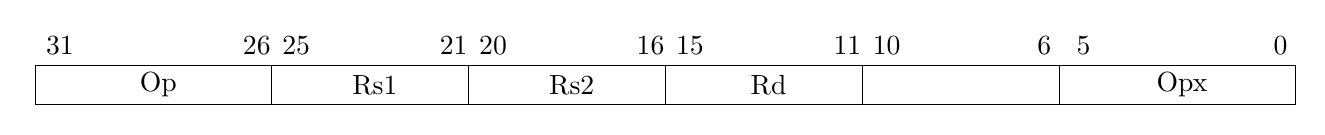
\begin{tikzpicture}[x=0.5cm, y=0.5cm]
                                \node at (0.5, 0.5) {~31~};
                                \node at (5.5, 0.5) {~26~};
                                \node at (6.5, 0.5) {~25~};
                                \node at (10.5, 0.5) {~21~};
                                \node at (11.5, 0.5) {~20~};
                                \node at (15.5, 0.5) {~16~};
                                \node at (16.5, 0.5) {~15~};
                                \node at (20.5, 0.5) {~11~};
                                \node at (21.5, 0.5) {~10~};
                                \node at (25.5, 0.5) {~6~};
                                \node at (26.5, 0.5) {~5~};
                                \node at (31.5, 0.5) {~0~};
                                \draw
                                (0, 0) -- (32, 0) -- (32, -1) -- (0, -1) -- cycle
                                (6, 0) -- (6, -1)
                                (11, 0) -- (11, -1)
                                (16, 0) -- (16, -1)
                                (21, 0) -- (21, -1)
                                (26, 0) -- (26, -1);
                                \node at (3, -0.5) {~Op~};
                                \node at (8.5, -0.5) {~Rs1~};
                                \node at (13.5, -0.5) {~Rs2~};
                                \node at (18.5, -0.5) {~Rd~};
                                \node at (29, -0.5) {~Opx~};
                            \end{tikzpicture}
                        \end{center}
                        For example, ~ADD R8, R6, R4~ sets the value of ~R8~ to be the sum of ~R6~ and ~R4~.
                    \item \textbf{register-immediate} \hfill one source and one destination register, immediate operand (e.g. adding)
                        \begin{center}
                            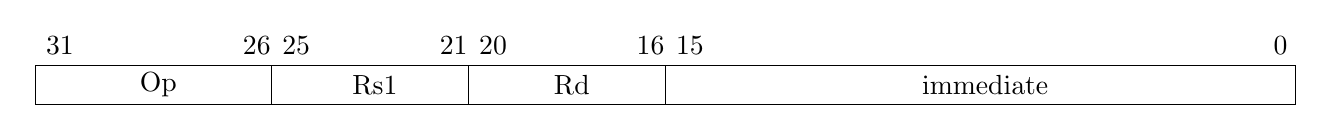
\begin{tikzpicture}[x=0.5cm, y=0.5cm]
                                \node at (0.5, 0.5) {~31~};
                                \node at (5.5, 0.5) {~26~};
                                \node at (6.5, 0.5) {~25~};
                                \node at (10.5, 0.5) {~21~};
                                \node at (11.5, 0.5) {~20~};
                                \node at (15.5, 0.5) {~16~};
                                \node at (16.5, 0.5) {~15~};
                                \node at (31.5, 0.5) {~0~};
                                \draw
                                (0, 0) -- (32, 0) -- (32, -1) -- (0, -1) -- cycle
                                (6, 0) -- (6, -1)
                                (11, 0) -- (11, -1)
                                (16, 0) -- (16, -1);
                                \node at (3, -0.5) {~Op~};
                                \node at (8.5, -0.5) {~Rs1~};
                                \node at (13.5, -0.5) {~Rd~};
                                \node at (24, -0.5) {~immediate~};
                            \end{tikzpicture}
                        \end{center}
                        Examples of this include;
                        \begin{itemize}
                            \itemsep0em
                            \item ~LW R2, 100(R3)~ \hfill ~R2 <- Memory[R3+100]~
                                \subitem source register is to be added to an immediate constant, could be useful for accessing fields of a struct (field offset is the constant) by using the base of the object
                            \item ~SW R5, 100(R6)~ \hfill ~Memory[R6+100] <- R5~
                                \subitem same as above, but for storing
                            \item ~ADDI R4, R5, 50~ \hfill ~R4 <- R5 + signExtend(50)~
                                \subitem note the sign extend; since we have a 16-bit immediate value, if it's a negative number, it needs to be padded to 32-bit
                        \end{itemize}
                    \item \textbf{branch}
                        \begin{center}
                            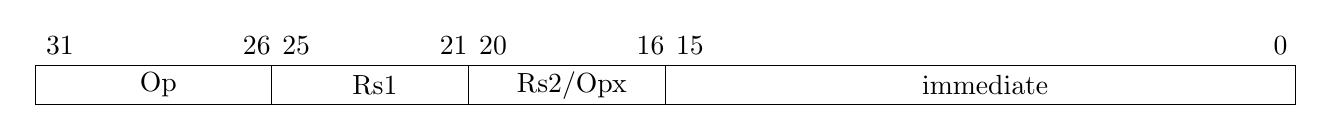
\begin{tikzpicture}[x=0.5cm, y=0.5cm]
                                \node at (0.5, 0.5) {~31~};
                                \node at (5.5, 0.5) {~26~};
                                \node at (6.5, 0.5) {~25~};
                                \node at (10.5, 0.5) {~21~};
                                \node at (11.5, 0.5) {~20~};
                                \node at (15.5, 0.5) {~16~};
                                \node at (16.5, 0.5) {~15~};
                                \node at (31.5, 0.5) {~0~};
                                \draw
                                (0, 0) -- (32, 0) -- (32, -1) -- (0, -1) -- cycle
                                (6, 0) -- (6, -1)
                                (11, 0) -- (11, -1)
                                (16, 0) -- (16, -1);
                                \node at (3, -0.5) {~Op~};
                                \node at (8.5, -0.5) {~Rs1~};
                                \node at (13.5, -0.5) {~Rs2/Opx~};
                                \node at (24, -0.5) {~immediate~};
                            \end{tikzpicture}
                        \end{center}
                        Two registers, for example if the contents are equal, then branch.
                        One challenge is that the address would have to fit in the immediate field, therefore it's not an \textbf{absolute} address, but one that's \textbf{relative} to the current program counter.
                        Note that it's multiplied by 4, as it's a fixed size.
                        For example, ~BEQ R5, R7, 25~; if ~R5 = R7~, then update ~PC <- PC + 4 + 25*4~, otherwise ~PC <- PC + 4~ (we update it regardless).
                    \item \textbf{jump / call}
                        \begin{center}
                            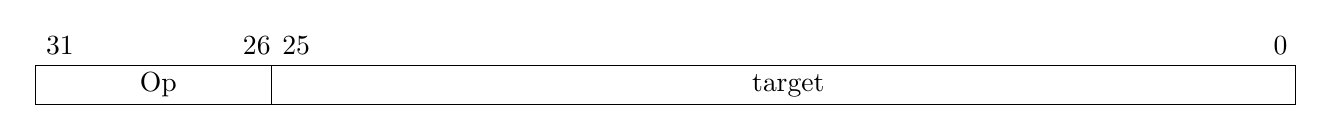
\begin{tikzpicture}[x=0.5cm, y=0.5cm]
                                \node at (0.5, 0.5) {~31~};
                                \node at (5.5, 0.5) {~26~};
                                \node at (6.5, 0.5) {~25~};
                                \node at (31.5, 0.5) {~0~};
                                \draw
                                (0, 0) -- (32, 0) -- (32, -1) -- (0, -1) -- cycle
                                (6, 0) -- (6, -1);
                                \node at (3, -0.5) {~Op~};
                                \node at (19, -0.5) {~target~};
                            \end{tikzpicture}
                        \end{center}
                        Unconditional branch, allowing for a jump to anywhere in the full address space of the machine.
                \end{itemize}
                The top bits are occupied by the opcode.
                Register specifier fields also occupy fixed positions in the instruction allowing immediate access to the registers before the instruction finishes decoding.
                In MIPS, we can have up to 32 registers in the machine as the width of the register specifier fields is 5 ($2^5 = 32$).
                The largest signed immediate operand is determined by the width of the immediate field, similarly the range of addresses of a conditional jump is the same (albeit scaled by 4).
                A general machine would execute this in a loop (the slides contain a diagram of this with the components);
                \begin{lstlisting}
                    Instr = Mem[PC]; PC += 4;
                    rs1 = Reg[Instr.rs1];
                    rs2 = Reg[Instr.rs2];
                    imm = signExtend(Instr.imm);
                    Operand1 = if (Instr.op == BRANCH) then PC else rs1
                    Operand2 = if (immediateOperand(Instr.op)) then imm else rs2
                    res = ALU(Instr.op, Operand1, Operand2)
                    switch (Instr.op) {
                      case BRANCH:
                        if (rs1 == 0) then PC = PC + imm*4; continue;
                      case STORE:
                        Mem[res] = rs1; continue
                      case LOAD:
                        Imd = Mem[res]
                    }
                    Reg[Instr.rd] = if (Instr.op == LOAD) then Imd else res
                \end{lstlisting}
                The 5 steps of the MIPS datapath are as follows - the pipelined design introduces pipeline buffers between each stage;
                \begin{enumerate}[1.]
                    \itemsep0em
                    \item instruction fetch
                    \item instruction decode, register fetch
                    \item execute, address calculation
                    \item memory access
                    \item write back
                \end{enumerate}
                The pipeline buffers allow the result of a stage to be latched in the buffer, to be used in the next clock cycle.
                This allows each instruction to progressively move down the pipeline on each successive clock tick.
                Without pipelining, the entire pipeline would operate on one clock cycle, however the number of gates along the path would determine the clock cycle time / rate - a non-pipelined processor would run slowly as there is a long path.
                In a pipelined design, the cycle time is determined by the slowest of the stages, but the length of each stage is controlled to allow for the highest possible rate.
                \medskip

                In addition to this, there is also a decode which controls what is being done (which sources to read from, for example a branch would use PC rather than a register).
                The control signals configure the multiplexers (MUX), ALU, and read / write to memory.
                The signal is carried with the corresponding instruction along the pipeline.
                \medskip

                Initially the pipeline is empty.
                With each successive cycle after the first, more of the pipeline will be used, with a new instruction being fetched at each cycle, and the preceding instruction being passed to the next pipeline stage.
                \medskip

                Pipeline doesn't make each individual instruction complete quicker; it doesn't help the \textbf{latency} of an instruction, but rather the \textbf{throughput} of the entire workload.
                The pipelining doesn't add much cost as we're using the same hardware, other than latches which add some transistor count and energy consumption.
                Adding more stages to a pipeline could lead to the clock rate being dominated by the time time the signal is spent in the latches.
                \medskip

                However, there are a number of hazards to pipelining;
                \begin{itemize}
                    \itemsep0em
                    \item \textbf{structural hazards} - particular hardware units may not be able to be used by two different pipeline stages in the same cycle
                        \smallskip

                        The \textit{PS3} was based on a highly parallel multi-core processor chip.
                        The processor had a conventional unit to run the Linux OS, but also 16 parallel accelerator units (fast but simple units, no cache, just a block of SRAM for instructions and data).
                        In cycle 4, for the first instruction, it would be accessing memory, however in the same cycle, a later instruction would be trying to fetch the instruction from the \textbf{same} memory.
                        A structural hazard occurs on simultaneous access; leading to load instructions causing an instruction fetch to stall.
                        This causes a stall (delays the instruction until the next cycle), which introduces pipeline bubbles - a missed opportunity for an instruction to be processed; once a fetch is missed, subsequent steps can't do anything in next cycles.
                        This was solved with a prefetch buffer, where a block of instructions was fetched at once.
                        Instructions were reorganised at compile time.
                    \item \textbf{data hazards} - an instruction depends on the result of an incomplete (still in pipeline) instruction (causes bubbles / stalls, can be overcome with forwarding)
                        \smallskip

                        Consider the following example;
                        \begin{lstlisting}
                            ADD R1,R2,R3
                            SUB R4,R1,R3
                            AND R6,R1,R7
                            OR R8,R1,R9
                            XOR R10,R1,R11
                        \end{lstlisting}
                        After the instruction is fetched in cycle one (for the ~ADD~), ~R2~ and ~R3~ are read in in cycle 2, available in cycle 4, but only written back in cycle 5.
                        For the ~SUB~ and ~AND~ instructions, the data would need to be sent back in time in the current idea of the pipeline, which obviously isn't feasible.
                        ~XOR~ is possible, as the register read is in cycle 6.
                        For ~OR~, this is fine \textbf{if} the register write happens in the first half of the clock cycle, and the register read happens in the second half.
                        \medskip

                        The previous assumption is that the value had to be written to the register before it could be used; however, at the end of cycle 3 the result of the ~ADD~ instruction is present in the latch after the execution stage, and could be fed directly into the ALU (same for the next instruction, but rather from the latch after the memory stage).
                        The value needs to be delayed by one clock cycle, before forwarding. % why?
                        \medskip

                        The changes to the hardware to support this are as follows (see lecture slides for diagrams);
                        \begin{itemize}
                            \itemsep0em
                            \item add forwarding / bypass paths (to the MUX, mentioned next)
                                \begin{itemize}
                                    \itemsep0em
                                    \item result of the ALU from previous cycle (latch)
                                    \item the latch after memory, for forwarding the value to the next instruction but one
                                    \item final wire takes value from memory
                                \end{itemize}
                            \item expand multiplexers before ALU to select where the operands should come from (choose one of the bypass wires if forwarding is needed)
                            \item decode needs to control bigger multiplexers to select values from bypass paths for forwarding; decode will now need to track which registers are going to be updated by incomplete instructions (the decode stage knows where the operands are going to come from, as well as what operands are still in-flight)
                        \end{itemize}
                        Data hazards can still exist even with forwarding, for example with loads, as the memory access comes later in the pipeline;
                        \begin{lstlisting}
                            LW R1,0(R2)
                            SUB R4,R1,R6
                            AND R6,R1,R7
                            OR R8,R1,R9
                        \end{lstlisting}
                        Recall that arithmetic may be involved to access memory, hence the stage has to come later.
                        For the value that is required in cycle 4 (execution of ~SUB~), the value is only available at the end of the cycle.
                        There is nothing that can be done here, leading to a bubble (also known as a load-use stall).
                        Stalls will also need to be implemented to support this.
                        \medskip

                        Software scheduling can be performed to avoid load hazards (recall that bubbles are missed opportunities for execution).
                        Consider the following code;
                        \begin{lstlisting}
                            a = b + c
                            d = e - f
                        \end{lstlisting}
                        Slow code, without the optimisation takes 10 cycles, with 2 stalls;
                        \begin{lstlisting}
                            LW    Rb,b
                            LW    Rc,c
                            STALL
                            ADD   Ra,Rb,Rc
                            SW    a,Ra
                            LW    Re,e
                            LW    Rf,f
                            STALL
                            SUB   Rd,Re,Rf
                            SW    d,Rd
                        \end{lstlisting}
                        However, the faster code swaps the order of execution by moving ~LW Re,e~ in place of the first stall and ~SW a,Ra~ in place of the second stall.
                        This takes 8 cycles and has no stalls;
                        \begin{lstlisting}
                            LW    Rb,b
                            LW    Rc,c
                            LW    Re,e
                            ADD   Ra,Rb,Rc
                            LW    Rf,f
                            SW    a,Ra
                            SUB   Rd,Re,Rf
                            SW    d,Rd
                        \end{lstlisting}
                    \item \textbf{control hazards} - we assume that we already know the next instruction to fetch, however this may not be the case as we haven't decoded the previous instruction yet (may be a jump / branch)
                        \smallskip

                        Consider the following example, where we may risk stalling for three cycles;
                        \begin{lstlisting}
                            BEQ R1,R3,36
                            AND R2,R3,R5
                            OR R6,R1,R7
                            ADD R8,R1,R9
                            XOR R10,R1,R11 # instruction 36
                        \end{lstlisting}
                        After discovering the branch outcome at cycle 3, we may suffer a bad stall.
                        This can be overcome by adding early branch determination.
                        Add an adder to add the current PC to the immediate operand (in decode stage), add check with with register file, and if it passes we can use the computed next PC value
                        All the logic for determining the branch outcome is moved as early as possible in the pipeline.
                        This still introduces a delay for one cycle, as we have to fetch the next instruction regardless (while we're computing whether we should branch or not).
                        If the branch is taken, the memory access and write back stages are blocked.
                \end{itemize}
                Simultaneous multi-threading can eliminate hazards.
                Without stalls, an instruction could be finished each cycle.
                Two program counters are maintained and the processing alternates between the two counters.
                Each thread has its own program counter and own registers, thus eliminating issues with data hazards (can still occur with memory).
                \medskip

                A simple pipeline with 5 stages can run at 5 - 9 GHz, limited by the \textbf{critical} path (slowest pipeline stage).
                The main tradeoff is to do more per cycle or to increase the clock rate.
            \subsection*{Introduction to Caches}
                In \textit{Intel Skylake}, there are L3 caches between the cores, an L2 cache associated with each individual core, as well as L1 data and instruction caches deeply embedded in the processor.
                In the past, RAM access time was close to the CPU's cycle time, hence there was little need for cache.
                However, the gap between the processor and the memory grows by around 50\% each year, leading to a growing gap (despite DRAM performance still increasing) - access times can be above 100 cycles.
                The lecture then goes into the memory hierarchy.
                \medskip

                Caches works due to the principal of locality, of which there are two types - most (if not all) modern architectures rely heavily on locality;
                \begin{itemize}
                    \itemsep0em
                    \item \textbf{temporal locality} - if an item is referenced, it will be used again soon (loops, reuse)
                    \item \textbf{spatial locality} - if an item is reference, items (addresses) close by tend to be used soon (straightline code, array access)
                \end{itemize}
                Consider a direct mapped cache, of size 1KB and blocks that are 32 bytes wide (32 blocks, as $1024 = 32 \times 32$).
                For a cache of size $2^N$ bytes, the uppermost $32 - N$ bits are the cache tag, with the lowest $M$ bits being the byte select (the block size is $2^M$);
                \begin{center}
                    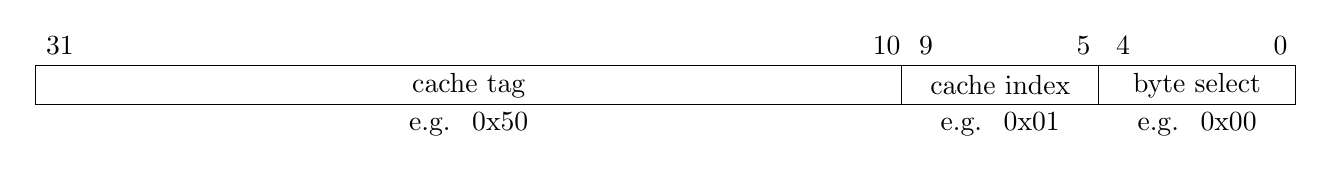
\begin{tikzpicture}[x=0.5cm, y=0.5cm]
                        \node at (0.5, 0.5) {~31~};
                        \node at (21.5, 0.5) {~10~};
                        \node at (22.5, 0.5) {~9~};
                        \node at (26.5, 0.5) {~5~};
                        \node at (27.5, 0.5) {~4~};
                        \node at (31.5, 0.5) {~0~};
                        \draw
                        (0, 0) -- (32, 0) -- (32, -1) -- (0, -1) -- cycle
                        (22, 0) -- (22, -1)
                        (27, 0) -- (27, -1);
                        \node at (11, -0.5) {cache tag};
                        \node at (11, -1.5) {e.g. ~0x50~};
                        \node at (24.5, -0.5) {cache index};
                        \node at (24.5, -1.5) {e.g. ~0x01~};
                        \node at (29.5, -0.5) {byte select};
                        \node at (29.5, -1.5) {e.g. ~0x00~};
                    \end{tikzpicture}
                \end{center}
                The example would select the second row (bytes 32 to 63), and take byte 32.
                \begin{center}
                    \begin{tabular}{|p{3cm}|p{3cm}|p{3cm}|p{3cm}|c}
                        \cline{1-4}
                        byte 31 & $\cdots$ & byte 1 & byte 0 & 0 \\
                        \cline{1-4}
                        byte 63 & $\cdots$ & byte 33 & \violet{byte 32} & 1 \\
                        \cline{1-4}
                        \multicolumn{4}{|c|}{$\vdots$} \\
                        \cline{1-4}
                        byte 1023 & $\cdots$ & byte 993 & byte 992 & 1 \\
                        \cline{1-4}
                    \end{tabular}
                \end{center}
                The role of the cache tag is to add metadata, including comparing the tag in the table with the tag in the cache.
                If it matches, and the valid bit is set, then we have a cache hit, otherwise a cache miss.
                \medskip

                This has a problem; cache location 0 can be occupied by data from main memory locations 0, 32, 64, and so on, similarly for location 1 being occupied by memory locations 1, 33, 65.
                Consider the following program, in C;
                \begin{lstlisting}
                    int A[256];
                    int B[256];
                    int r = 0;
                    for (int i = 0; i < 10; ++i) {
                      for (int j = 0; j < 64; ++j) {
                        r += A[j] + B[j];
                      }
                    }
                \end{lstlisting}
                The memory will be allocated contiguously, each being 256 bytes (or 8 32 byte cache lines).
                The 1KB direct-map cache should be able to hold all the integers (as it's only a total of 512B).
                However; ~A[0]~ and ~B[0]~ would have identical address bits (for the cache index) - since they are exactly 1024 bytes apart, meaning they will map to the same place, as well as all subsequent values.
                This means they will continuously displace each other, and only use a subset of the cache.
                \medskip

                This is solved with an associative cache - for an $N$-way set associative cache, there are $N$ entries for each cache index (typically 2 to 4); $N$ direct mapped caches operated in parallel.
                The cache index selects a set from the cache, the two tags are compared, and the data is selected based on the matching tag result (if either leads to a hit, it's a hit, otherwise a miss).
                \medskip

                However, this leads to adding extra hardware, which is on the \textbf{critical path} for determining whether it's a cache hit or miss (adding an additional MUX introduces another gate delay, which we already have few of).
                \medskip

                An example is the \textit{Intel Pentium 4 Level-1 Cache}.
                This had a capacity of 8KB (total data it can store), blocks of size 64 bytes (128 blocks in the cache), $N = 4$ (4-way set associative cache), leading to 32 sets.
                The index was 5 bits, to select one of the 32 sets, leading to a tag of 21 bits ($32 - 5 - 6$, subtracting the index and the 6 to address the byte within the block).
                The access time of this was 2 cycles.
                \medskip

                There are 4 questions for memory hierarchy;
                \begin{enumerate}[1.]
                    \itemsep0em
                    \item where can a block be placed in the upper level? \hfill \textbf{block placement}
                        \smallskip

                        In a direct-mapped cache, there is only one cache location it can be placed in, determined by its low-order address bits.
                        In an 2-way set-associative cache, it can be placed in either of the two cache locations corresponding to the set determined by low-order address bits.
                        A fully-associative cache, it can be placed in any location - more associativity leads to the issues;
                        \begin{itemize}
                            \itemsep0em
                            \item more comparisons (more transistors, more energy, larger)
                            \item better hit rate (a lot of associativity leads to diminishing returns)
                            \item more predictable; reduced storage layout sensitivity (cache hits are independent of storage layout)
                        \end{itemize}
                    \item how is a block found if it's in the upper level \hfill \textbf{block identification}
                        \smallskip

                        In addition to the memory required to store the cached data, we need metadata (valid, cache tag) to tell us whether we have a hit or not.
                        The tag doesn't need to include the block offset nor the cache index.
                        As associativity increases, the index shrinks (less indices) and expands the tag.
                    \item which blocks should be replaced on a miss? \hfill \textbf{block replacement}
                        \smallskip

                        In a direct-mapped cache, there is no choice to be made, and it can only replace one block.
                        However, with an associative cache we ideally want to choose to replace the block that will be reused least-soon.
                        LRU (least recently used) is a good approximation, random is very good for large caches (LRU only beats random for small caches).
                        A program that periodically sweeps over an array that doesn't fully fit into cache would be bad in LRU.
                    \item what happens on a write? \hfill \textbf{write strategy}
                        \smallskip

                        On a store instruction, we need to check if that address is cached.
                        If it is, then we must update it.
                        However, we need to decide whether to write to the next level of the memory hierarchy (write through), main memory, or not (write back).
                        The latter only updates the cache and not the next level of the hierarchy \textbf{until} the block is evicted (replaced) - this requires an additional status bit to indicate whether the block is clean or dirty.
                        The write back strategy has an advantage with repeated writes to the same location as the writes are absorbed without propagating to main memory - this may include writing to successive elements in an array.
                        Write through ensures the rest of the system gets updated more promptly.
                        This helps with cache coherency, however it does not solve it entirely, as other processes may have their own cached copies of this data.
                \end{enumerate}
                The lecture then continues about the bottom of the memory hierarchy (large machines with robot arms for tapes), as well as architectures that don't have caches and therefore don't depend on locality in access patterns.
                The latter has the idea that with enough threads, memory latency can be hidden.
            \subsection*{Turing Tax Discussion}
                A stored-program computer is a machine that fetches instructions from memory and executes them.
                \textit{John Backus} dubbed the limitation of the stored-program mode being serial (one instruction at a time) the \textit{von Neumann bottleneck}, and suggested writing our programs in a way that expresses the data dependencies without prematurely committing to the exact order the instructions should be executed in (functional programming).
                \medskip

                \textit{Alan Turing} proposed the idea of a universal / single device which can implement any computable function without further configuration, given the right program.
                The tax refers to the overhead for execution time, manufacturing cost of the machine, or the energy required for computation.
                The aim is to characterise the cost difference between programming a general purpose machine to do a job, versus designing a application-specific machine for it.
                \medskip

                H.264 encoding is dominated by 5 stages, applied to a stream of macroblocks (blocks of the video) - the remaining steps correspond to finding a compact encoding;
                \begin{enumerate}[(i)]
                    \itemsep0em
                    \item \textbf{IME} Integer Motion Estimation \hfill motion relative to previous frame
                    \item \textbf{FME} Fractional Motion Estimation \hfill refines the previous estimate
                    \item \textbf{IP} Intra Prediction
                    \item \textbf{DCT/Quant} Transform and Quantisation
                    \item \textbf{CABAC} Context Adaptive Binary Arithmetic Coding
                \end{enumerate}
                An ASIC, fully customised for this task, was able to outperform \textit{Intel Pentium} at a significantly lower energy consumption and smaller size.
                \medskip

                Turing Tax is present in our pipeline in many stages.
                The instruction fetch, maintaining PC, handling and predicting branches are all tasks that could be avoided in a specialised machine.
                Routing paths be replaced by colocating the producer and consumer together, shortening wires.
                Registers are also used to pass instructions from one instruction to the next; in a special-purpose machine, this can be a single piece of wire connecting units.
                The ALU can be configured to do many different things in our pipeline, but in a specialised machine, we may have several ALUs, each specific to a particular operation.
        \subsection*{Chapter 2}
            \subsubsection*{Dynamic Scheduling, Out-of-order Execution, Register Renaming}
                Consider the following instructions;
                \begin{lstlisting}
                    DIVD F0,F2,F4
                    ADDD F10,F0,F8
                    SUBD F12,F8,F14
                \end{lstlisting}
                Note that division can take many cycles (and is slow) and that the ~SUBD~ instruction doesn't use anything in either of the preceding instructions.
                The key idea is to allow an instruction that is behind a stall to proceed.
                \medskip

                There are a number of constraints on execution order (note that anything in ~monospace~ denotes an instruction, ~I~ refers to instruction ~I~);
                \begin{enumerate}[1.]
                    \itemsep0em
                    \item ~J~ is \textbf{data dependent} on ~I~ if ~J~ tries to read an operand before ~I~ writes it;
                        \begin{lstlisting}
                            I: ADD R1,R2,R3
                            J: SUB R4,R1,R3
                        \end{lstlisting}
                        It can also be the case that ~J~ is data dependent on ~K~ which is dependent on ~I~.
                        A Read After Write hazard is when a true dependence causes a hazard in the pipeline.
                    \item There are two types of \textbf{name dependence}, both of which have instructions that use the same register / memory location (called a name)
                        \begin{lstlisting}
                            I: SUB R4,R1,R3
                            J: ADD R1,R2,R3
                            K: MUL R6,R1,R7
                        \end{lstlisting}
                        The first kind is anti-dependence / Write After Read, where ~J~ writes an operand before ~I~ reads it, caused by the reuse of name ~R1~.
                    \item The second type is called an \textbf{output dependence}, where ~J~ writes the operand before ~I~ does;
                        \begin{lstlisting}
                            I: SUB R1,R4,R3
                            J: ADD R1,R2,R3
                            K: MUL R6,R1,R7
                        \end{lstlisting}
                        ~K~ needs to get the correct ~R1~, also called a Write After Write hazard.
                \end{enumerate}
                The decode stage can be renamed to issue; which decodes the instruction and checks for any structural hazards.
                There will also be a later read operands stage, where the operands are actually collected.
                In the issue stage, the register ~F0~ is checked and we may see that it's marked with some bit that indicates the value isn't ready yet and is being computed by an instruction that's in-flight.
                This stage may collect the operands if they are already available, otherwise discover where they will come from and collect it later in the read operands step.
                \medskip

                The lecture goes into the \textit{IBM 360/91}, which had a small number of FP registers in the instruction set.
                This prevented compiler scheduling for avoiding load-use stalls.
                \medskip

                Consider the following series of instructions, at the issue stage (multiply ~F1~ and ~F2~ into ~F0~, store into address ~X~, and similar for the next two instructions);
                \begin{lstlisting}
                    MUL F0,F1,F2
                    SD F0,X
                    MUL F0,F2,F3
                    SD F0,Y
                \end{lstlisting}
                The issue stage consults the registers and allocates the instruction being issued to a reservation station.
                The reservation station for each functional unit holds the opcode and the two operands; both of which need to be present before the instruction can progress to the functional unit.
                The registers can hold a value and tags (different to the ones we saw in cache); if the tag is null, then the value is valid (for example, the tag for ~F0~ would be null if no instruction in the machine is producing a value for ~F0~).
                If it isn't null, then it will indicate the ID of the functional unit that will produce the result for that register.
                \medskip

                In our example, there are 4 registers ~F0~ to ~F3~ and 4 reservation stations (~MUL1~, ~MUL2~, ~Store1~, ~Store2~).
                Going through the instructions;
                \begin{enumerate}[1.]
                    \itemsep0em
                    \item issue unit looks at instruction 1 and collects the operands from the source registers ~F1~ and ~F2~ (assume no instructions in the machine currently; the tag is null and the value is present)
                    \item allocate the multiply operation to the first unit ~MUL1~ by copying the values from ~F1~ and ~F2~, and update ~F0~ with the ID of the multiply unit (~MUL1~)
                    \item issue looks at instruction 2 and sees ~F0~ is waiting for ~MUL1~
                    \item allocate the operation to ~Store1~ by copying in the tag ~MUL1~
                    \item issue looks at instruction 3 and collects the results from the source registers, which are present
                    \item allocate the operation to ~MUL2~, and overwrite ~F0~ with the ID of the unit ~MUL2~
                    \item similar for the second store, but keeps the tag ~MUL2~ in the reservation station
                \end{enumerate}
                There is a common data bus that connects the results of the functional units to \textbf{both} the registers as well as the reservation stations.
                When ~MUL1~ finishes, a signal is sent and anything listening for that tag will be updated - since ~Store1~ had the tag from the registers and is waiting on ~MUL1~, it would get the value.
                On the other hand, if ~MUL2~ were to somehow finish before, it would update the value in the register (as well as the ~Store2~ reservation station), but not the ~Store1~ reservation station.
                \medskip

                We typically think of registers as a location where data is stored, but in the \textit{Tomasulo} design, the register becomes a tag that connects the production of the value to where it needs to be delivered to.
                At issue time, we are decoding the dependent structure of the program dynamically, and arranging for the forwarding wiring to deliver resulting operands to the functional units at the right time.
                \medskip

                Another walkthrough of the same instructions is as follows.
                Assume that the value fields of ~F1~ and ~F2~ are already populated;
                \begin{enumerate}[1.]
                    \itemsep0em
                    \item instruction 1 issued; \textbf{values} of ~F1~ and ~F2~ are routed to ~MUL1~'s operands 1 and 2 respectively, as both tags are null, the tag of ~F0~ is updated with ID of ~MUL1~, stating that the value will come from there
                    \item instruction 2 issued; \textbf{tag} of ~F0~ (~MUL1~) is routed to ~Store1~ as well as address ~X~
                    \item instruction 3 issued; \textbf{values} of ~F2~ and ~F3~ routed to ~MUL2~'s operands (since both tags are null again), and tag of ~F0~ is \textbf{overwritten} with ID of ~MUL2~, updating where the value will come from
                    \item instruction 4 issued; \textbf{tag} of ~F0~ (~MUL2~) is routed to ~Store2~ as well as address ~Y~
                    \item at this point, nothing has completed yet; both store units are waiting for a value matching the tag to be broadcasted on the common data bus, ~F0~ is also waiting
                    \item ~MUL1~ finishes; broadcasts the result on CDB with the ~MUL1~ tag - ~Store1~ picks up the value and stores to memory, ~F0~ doesn't do anything as it's now waiting for ~MUL2~
                    \item ~MUL2~ finishes; also does the broadcast, picked up by ~Store2~ which stores to memory, ~F0~ also updates its value
                \end{enumerate}
                There are three stages of this algorithm;
                \begin{enumerate}[1.]
                    \itemsep0em
                    \item \textbf{issue}
                        \smallskip

                        Gets the instruction from FP operation queue.
                        If the reservation station is free (hence no structural hazard), the instruction is issued and operands are sent (renaming registers).
                    \item \textbf{execute}
                        \smallskip

                        Actually operands on operands when \textbf{both} operands are ready.
                        If they aren't both ready, then watch the CDB for a result.
                    \item \textbf{write result}
                        \smallskip

                        Write to the CDB for all units that are waiting, and also mark the RS as available.
                \end{enumerate}
                This relies on two busses, the first data bus which goes from issue to the registers, as well as the common data bus which goes from the functional units to the reservation stations as well as the registers.
                \medskip

                However, this design is complex, leading to many comparators on the common data bus.
                The CDB also limits performance as it needs to connect multiple functional units to multiple destinations - the number of functional units that can complete per cycle is dependent on the number of CDBs (one in our case).
                Finally, the trickiest issue is non-precise interrupts.
                \medskip

                As a loop is essentially the same instructions, a compiler wold have to introduce new registers to be able to find a static schedule.
                The scheme effectively implements register renaming.
                Consider the following example with a loop (load using ~R1~ as a pointer, multiply with that result with some constant into ~F4~ and store it into the same place, then decrement the pointer down to zero);
                \begin{lstlisting}
                    Loop:
                        LD      F0 0(R1)
                        MULTD   F4 F0 F2
                        SD      F4 0(R1)
                        SUBI    R1 R1 #8
                        BNEZ R1 Loop
                \end{lstlisting}
                Assume multiply takes 4 cycles, loads take 8 cycles (misses the L1 cache, hits L2 cache), assume integer instructions and store instructions don't use the CDB.
                See the slides for the actual pipeline; but it essentially allows for four iterations of the loop to be running (in-flight) in parallel with each other.
                A more realistic scenario is that the second iteration has a hit on the L1 cache, which dynamically adapts the schedule based on cache hits / misses, something that is very valuable in dynamic scheduling.
            \subsubsection*{Speculation in Dynamically-scheduled Processors}
                On a conditional jump, we don't have to wait, but rather take a guess which gives us much higher performance if correct and handle the case if not.
                With a misprediction, we need to roll-back the state to the state before the prediction.
                This is done by adding a stage to the Tomasulo execution pipeline to commit the state of the machine.
                The speculative Tomasulo algorithm is as follows (a branch misprediction would flush this buffer);
                \begin{enumerate}[1.]
                    \itemsep0em
                    \item \textbf{issue}
                        \smallskip

                        If the reservation station (and the reorder buffer slot) is free, issue instruction, send operands and reorder buffer number for destination.
                        One ROB entry is allocated for each instruction, and this holds the destination register with either its result value (or the tag from where it will come from).
                    \item \textbf{execute} \hfill same as before
                    \item \textbf{write result}
                        \smallskip

                        Write to all awaiting units and reorder buffer (also marks RS as free).
                        A ROB entry with the matching tag is also updated.
                    \item \textbf{commit}
                        \smallskip

                        This updates the register with the reorder result.
                        When an instruction is at the head of the buffer and has a present result; the commit-side register (or stored to memory) is updated with result, and instruction is removed from the reorder buffer.
                \end{enumerate}
                The existing machine is extended with the buffer, the commit unit, and commit-side registers.
                The issue stage pushes instructions onto the buffer, which listens to results on the CDB, and the commit unit commits the results in \textbf{program order}.
                The only externally visible part of this machine is the commit-side registers (updated when the speculation is resolved); if we want to reset to a previous stage, we only look at what's on the committed side of the machine.
                Previously, we only had the issue-side registers (which were updated speculatively).
                \medskip

                Consider an example as follows (assume that we predict the branch isn't taken);
                \begin{lstlisting}
                    MUL F0,F1,F2
                    SD F0,X
                    BEQ R10,Lab
                    MUL F0,F2,F3
                    SD F0,Y
                \end{lstlisting}
                Note that the ROB would be in the same order as the instructions, and we would also store the prediction in the ROB (for ~BEQ~).
                By the time the first two are committed, and ~BEQ~ is at the head of the buffer, assume we also have the result for ~BEQ~.
                This is compared to our prediction - consider a misprediction; all subsequent entries in the ROB are trashed, the issue-side registers are reset using values from the commit-side registers (as they are correct even before the misprediction), and finally the correct target instruction is fetched and issued.
                As such, we reinstate the register state at the point the conditional branch was executed.
                Due to this, we can see a penalty as we are discarding work that has been done and we also need to refill the pipeline.
                Assume that the FUs are still working - once they complete and write back, nothing will be waiting (ROB is flushed, as well as issue-side registers).
                \medskip

                One subtlety that could be considered is the case where we know the branch is mispredicted before it's at the head of the buffer.
                We could start to fetch the correct instruction, however we need to take care to ensure that we are in a consistent state.
                Another case is when there are two predicted branches; the current approach will handle this fine as the entire ROB is flushed once the first prediction is at the head, and turns out to be a misprediction.
                \medskip

                Another subtlety lies in stores buffered in the ROB; it's important to buffer them before writing to the memory system.
                However if something attempts to load from that memory location, the correct data may not be in memory yet.
                A conservative strategy for this could be to stall loads until preceding stores have all been completed.
                Another approach would be to check all preceding store instructions for the address in memory (even if it's one that is waiting to be computed) - if none of them match the load instruction's target, then the load can take place.
                We would need to stall loads until all addresses are known for preceding instructions.
                If it matches the address of an uncommitted store, the data can simply be forwarded to the load - care should be taken to ensure we take from the most recent store (in the case multiple instructions are writing to the same address).
                \medskip

                Stores and loads use computed addresses, which may not be known at issue time (unlike registers).
                Consider the following;
                \begin{lstlisting}
                    SD F0,0(R3) ; store F0 at address R3
                    LD R2,0(R1) ; load address from memory
                    SD F1,0(R2) ; store F1 to that address
                    LD F2,0(R3) ; load F1 from address R3
                \end{lstlisting}
                However, we don't know until instruction 2 has finished executing whether ~R1 = R3~.
                We could predict that it doesn't match, and directly forward ~F0~ to ~F2~ from instruction 1 to 4 - if this is correct, we obtain a significant performance improvement (store-to-load forwarding).
                \medskip

                There are alternatives for out-of-order processor architectures, we will look at the register update unit (RUU) versus ROB.
                The RUU essentially unifies the ROB and reservation stations.
                When the instructions are ready to run (operands populated), the dispatcher selects the next ready entry and dispatches it to a functional unit.
                The decision is deferred to the dispatch unit, rather than going directly to the reservation station for a functional unit.
                Note that the tags correspond to the indices in the RUU, rather than to each functional unit as before.
                As such, the ROB entry acts as renamed register for the instruction's result.
                \medskip

                \textit{Pentium III} attempted to reduce the amount of copying.
                The register alias table tracks the latest alias for logical registers (pointing to ROB or RRF (retired register file) - would've been commit-side registers in our previous example).
                Once retired, the pointer is switched to one in the RRF.
                In \textit{Pentium 4 / NetBurst}, this is more explicit as there are two RATs (frontend and retirement) - the committed state of the machine is represented by the physical registers in the RF (register file, entirely dynamic) pointed to by the retirement RAT.
                \medskip

                Watch the end of the lecture for details on \textit{Pentium 4}.
                \medskip

                In conclusion, dynamic scheduling reduces the dependence on the compiler scheduling instructions (and the compiler's knowledge of the hardware - compiler can generate code without knowing which processor the code is running on).
                It also handles dynamic stalls (for example cache misses, that the compiler would not know about in advance).
                Register renaming maps the limited number of registers in the instruction set to a much larger set of physical registers in the machine.
                However, this adds a considerable increase in the pipeline depth.
                Branch misprediction has higher latency.
                The complexity (and risk of error) is increased, as well as power consumption.
                Performance can also be difficult to understand.
        \subsection*{October 19 - Live Lecture}
            Consider a program for no temporal locality, or one without spatial locality.
            An example of the former is one that never revisits data, such as something that deals with a stream of data (once it's dealt with, it's never seen again); a simple example is summing an array (assuming we've never seen the data before so it isn't already in cache).
            A specific example of the latter is an array of structs where the entire struct fills the cache, but only a single field is used from each struct.
            Another example would be a large (larger than the cache) hash table - despite the `constant' access times.
            If the memory accesses are deliberately random (with little reuse), a tree structure may even be more beneficial.
            \medskip

            In a fully associative cache, the cache index bits are unused.
            Instead we basically scan the tag bits for every cache location, for every access.
            These are expensive as many comparators are required for \textbf{every} access.
            The MUX on the critical path could potentially become a clock rate limiting problem.
            The memory stage (and instruction fetch) could likely be the clock rate limiting stage due to slower memory accesses.
            \medskip

            Similar structures and issues found in caches will be found in branch prediction, prefetching, and so on.
            \medskip

            Consider the following code, which adds a scalar to a vector;
            \begin{lstlisting}
                for (i=1000; i >= 0; i=i-1)
                  x[i] = x[i] + s;
            \end{lstlisting}
            Translated into MIPS, we have the following (assuming 8 is the lowest address).
            Note that it takes 9 clock cycles per iteration;
            \begin{lstlisting}
                Loop: L.D    F0,0(R1) ; 1 stall
                      ADD.D  F4,F0,F2 ; 2 stalls
                      S.D    0(R1),F4
                      DSUBUI R1,R1,8
                      BNEZ   R1,Loop
                      NOP             ; delayed branch slot / stall
            \end{lstlisting}
            This could be rescheduled to the following, to have 6 cycles (albeit 3 of these are used for the loop overhead);
            \begin{lstlisting}
                Loop: L.D    F0,0(R1) ; 1 stall
                      ADD.D  F4,F0,F2
                      DSUBUI R1,R1,8
                      BNEZ   R1,Loop
                      S.D    8(R1),F4 ; this is altered since it's after DSUBUI
            \end{lstlisting}
            The program can be modified by unrolling the loop (each iteration does 4 steps);
            \begin{lstlisting}
                Loop: L.D    F0,0(R1)
                      ADD.D  F4,F0,F2
                      S.D    0(R1),F4
                      L.D    F0,-8(R1)
                      ADD.D  F4,F0,F2
                      S.D    -8(R1),F4
                      L.D    F0,-16(R1)
                      ADD.D  F4,F0,F2
                      S.D    -16(R1),F4
                      L.D    F0,-24(R1)
                      ADD.D  F4,F0,F2
                      S.D    -24(R1),F4
                      DSUBUI R1,R1,#32
                      BNEZ   R1,Loop
                      NOP
            \end{lstlisting}
            Our opportunities for rescheduling is limited by register reuse.
            This can be resolved by giving each copy of the loop a fresh set of registers (each copy of load, add, store uses a new set of registers).
            This moves all loads to the start, where enough time would have elapsed by the time we want to perform the additions (note that the expected ~-24(R1)~ has changed as it's after the ~DSUBUI~, as ~8 - 32 = -24~) - this becomes 3.5 cycles per iteration;
            \begin{lstlisting}
                Loop: L.D    F0,0(R1)
                      L.D    F6,-8(R1)
                      L.D    F10,-16(R1)
                      L.D    F14,-24(R1)
                      ADD.D  F4,F0,F2
                      ADD.D  F8,F6,F2
                      ADD.D  F12,F10,F2
                      ADD.D  F16,F14,F2
                      S.D    0(R1),F4
                      S.D    -8(R1),F8
                      S.D    -16(R1),F12
                      DSUBUI R1,R1,#32
                      BNEZ   R1,Loop
                      S.D    8(R1),F16
            \end{lstlisting}
            Suppose all reservation stations are occupied.
            The issue is that we have nowhere to now put the instructions, leading to a stall at the issue stage.
            As the issue stage is an in-order stage, this prevents overtaking (for example, if later instructions don't require the `full' reservation stations they won't be seen).
            These reservation stations are a factor for performance.
            \medskip

            The difference between ~MM1~ and ~MM2~ is the order of the matrix multiply; the former uses ~i,j,k~ whereas ~MM2~ uses ~i,k,j~.
            The latter is better as the compiler lays out the array row-by-row (in the former, the ~B[k][j]~ isn't walking down a row, even though ~C[i][j]~ is).
            This is important as we're able to use spatial locality in ~MM2~ (we will use all the elements in the cache block before going to the next one).
            On the other hand ~MM2~ and ~MM3~ splits the ~j~ and ~k~ loops, where ~jj~ and ~kk~ jump by ~blocksize~.
            The inner part of ~MM3~ still remains ~i,k,j~ (albeit doing the multiplication in smaller blocks) - known as loop tiling.
            By using tiles, we get around the issue of displacing tiles that we will use again in matrix multiplication.
            \medskip

            Registers are not places to store data, but rather indicate data flow (a special-purpose machine would have a wire connecting units).
            The ALU is controlled by a signal derived from decoding the instruction (it is multipurpose).
            However, in a specialised design, we'd likely have exactly the right number of required functional units.
            In a specialised machine, you'd know what's in cache locations (you'd have cache data, but not the tags) - the existence of cache isn't Turing Tax, but specific choices are.
            Architects avoid Turing Tax in a number of ways, including SIMD (which amortises the fetch-execute over a vector of operands), more complex instructions (macro-instructions), long cache lines, direct memory access, etc.
            Compilers also help by vectorising instructions, and so on.
        \subsection*{Chapter 3}
            Control hazards are present in any pipelined processor; we will likely need to know what instruction to fetch even before the current instruction has been evaluated, or even decoded.
            Branches are typically quite frequent, but can vary depending on the type of program.
            Amdahl's law suggests that whatever can't be accelerated becomes dominant, when everything else has been accelerated.
            Speculative dynamic instruction scheduling, along with register renaming, allows us to speculate many instructions, even through several branches.
            Not only is it important for branches, but other parts of the processor architecture can also benefit from hardware support for dynamic prediction.
            Virtual function calls (in a polymorphic language) can also depend on the context and may vary from invocation to invocation - they are also indirect jumps.
            \medskip

            Alternatives for branch prediction include;
            \begin{itemize}
                \itemsep0em
                \item \textbf{multithreading}
                    \smallskip

                    Suppose we have a simple 5 stage pipeline and 4 threads per core.
                    As such there are 4 PCs and 4 sets of registers.
                    By the time thread 0 is executing again in the fetch stage, we would've already determined the outcome of the first instruction - it should've completed the ALU stage.
                    With enough threads, the entire control problem disappears - however we care about the performance of individual threads.
                \item \textbf{predication}
                    \smallskip

                    Predication extends the instruction set by loading condition values into predicate registers (single bit).
                    For example, the simple code ~if (x == 10) c = c + 1;~ could become the following;
                    \begin{lstlisting}
                        :
                             LDR r5, X
                             p1 <- r5 eq 10
                        <p1> LDR r1 <- C
                        <p1> ADD r1, r1, 1
                        <p1> STR r1 -> C
                        :
                    \end{lstlisting}
                    The conditional body consists of instructions guarded by these conditional predicate registers.
                    The control hazard is converted into a data hazard.
                    By doing this, we avoid conditional branches, however this may be unattractive for large bodies of code - it would be better to jump over the entire body rather than fetching and decoding, and then realising the predicate is false.
                    It also eliminates the risk of a misprediction.
                \item \textbf{branch delays}
                    \smallskip

                    The branch instruction is redefined to take place after a following instruction.
                    \begin{center}
                        \vspace{-1.5\baselineskip}
                        \begin{minipage}[t]{0.31\textwidth}
                            \begin{lstlisting}
                                # source code
                                if (R1 == 0)
                                  X = 100
                                else
                                  X = 200
                                R5 = X
                            \end{lstlisting}
                        \end{minipage}
                        \begin{minipage}[t]{0.31\textwidth}
                            \begin{lstlisting}
                                # assembly code
                                  LW R3,#100
                                  LW R4,#200
                                  BEQZ R1,L1
                                  SW R3,X
                                  SW R4,X
                                L1:
                                  LW R5,X
                            \end{lstlisting}
                        \end{minipage}
                        \begin{minipage}[t]{0.31\textwidth}
                            \begin{lstlisting}
                                # what it does
                                if (R1 == 0)
                                  X = 100
                                else
                                  X = 100
                                  X = 200
                                R5 = X
                            \end{lstlisting}
                        \end{minipage}
                    \end{center}
                    The instruction after the branch ~SW R3,X~ is executed regardless; it's already been fetched.
                    If we are branching, then we go to ~L1~ after it's executed, otherwise we proceed to ~SW R4,X~.
                    For MIPS, it's sufficient to have a single delay slot.
                    \medskip

                    Ideally, we take an instruction from before the branch instruction.
                    Alternatively, we can take an instruction from either the target address, or from the fall through (although this is only valuable when it's correct) - we also want to ensure that it's the correct thing to do (hence we shouldn't store to memory, as we may store something that shouldn't be stored).
                    The performance of this can be improved with `cancelling' branches, with variants for whether the branch is likely taken or not.
                    With these instructions, the write-back is disabled if it wasn't supposed to be executed.
            \end{itemize}
            Ideally, with a branch predictor, we want to fetch the correct next instruction without stalling.
            Therefore, we need a prediction before the preceding instruction has even been decoded.
            There are two types of branches (conditional branches) which is direction prediction (whether it's taken or not), and indirect branches which is target prediction (definitely taken, an example of which is a branch to an address stored in a register, commonly present as virtual function calls or return addresses which is taken from the stack).
            \subsubsection*{Branch Direction Prediction (Takenness)}
                The simplest idea is to keep a table for each branch containing a bit representing whether it was taken or not last time (branch history table - BHT).
                If we take the $k$ lowest bits from the program counter to index a table of $2^k$ size.
                Once an instruction is completed, we update the corresponding entry with a 1 or 0 depending on whether it was supposed to be taken or not.
                One limitation of this is that the table is of limited size, hence multiple branch instructions may map to the same entry - same issue as associativity conflicts.
                A simple example where this may have issues is a nested loop; the first iteration of the inner loop will likely miss, as well as the last iteration of the inner loop (would've had taken in the BHT for the previous iterations, but this will fall through and update to not taken).
                The next iteration of the outer loop will also cause a miss in the inner loop (since the branch is taken, but the BHT suggests it won't be taken, as it fell through last time).
                \medskip

                A solution to the previous idea is to add hysteresis by having a second bit.
                This scheme only changes the prediction of there are two mispredictions (\violet{violet} represents predict taken and \teal{teal} represents predict not taken);
                \begin{center}
                    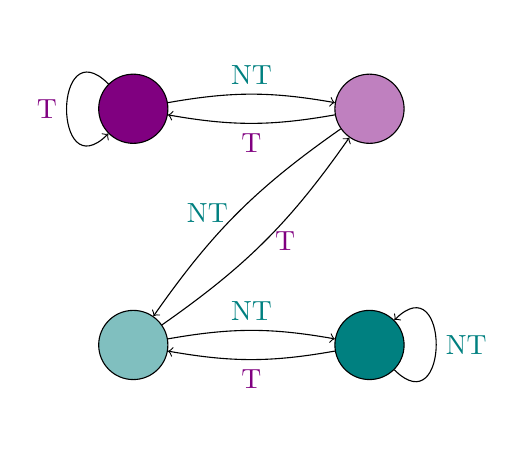
\begin{tikzpicture}
                        \node[state, fill=violet] (t) at (0, 0) {};
                        \node[state, fill=violet!50] (th) at (3, 0) {};
                        \node[state, fill=teal!50] (nth) at (0, -3) {};
                        \node[state, fill=teal] (nt) at (3, -3) {};

                        \draw
                        (t) edge[->, loop, left, out=135, in=225, distance=1cm] node{\violet{T}} (t)
                        (t) edge[->, bend left=10, above] node{\teal{NT}} (th)
                        (th) edge[->, bend left=10, below] node{\violet{T}} (t)
                        (th) edge[->, bend right=10, left] node{\teal{NT}} (nth)
                        (nth) edge[->, bend right=10, right] node{\violet{T}} (th)
                        (nth) edge[->, bend left=10, above] node{\teal{NT}} (nt)
                        (nt) edge[->, bend left=10, below] node{\violet{T}} (nth)
                        (nt) edge[->, loop, right, out=-45, in=45, distance=1cm] node{\teal{NT}} (nt);
                    \end{tikzpicture}
                \end{center}
                This idea also generalises to higher bit BHTs.
                Generally, the 2-bit predictor is often very good but can sometimes be quite awful.
                1-bit is usually worse, and 3-bit isn't usefully better.
                This is based on a saturating counter.
                Most branches are biased; they are either almost always taken or almost always not; this doesn't work for branches which aren't biased.
                The predictor is often called the bimodal predictor (two clusters).
                \medskip

                The bimodal predictor uses local history; the prediction is determined only by a memory address.
                Consider the following code, with three conditions;
                \begin{lstlisting}
                    if (C1) then
                      S1;
                    endif
                    if (C2) then
                      S2;
                    endif
                    if (C3) then
                      S3;
                    endif
                \end{lstlisting}
                It's likely that the conditions are correlated; for example, we may not know ~C1~, but once we do, we may know ~C2~ and ~C3~.
                We define the \textbf{global history} as the taken / not-taken history for all previous branches.
                The idea is to keep an $m$-bit branch history register (BHR), which is a shift register (push a zero or one) recording the taken / not-taken direction of the most recent $m$ branches.
                \medskip

                Consider an $(m, n)$ ``gselect'' predictor.
                There are $m$ global bits (BHR) recording the behaviour of the last $m$ branches which is used to select which of the $2^m$ $n$-bit BHTs to use.
                A popular choice is $m = n = 2$, hence there are 4 tables of $2 \times 2^k$ bits.
                The update is also done based on the same BHR, so a different history would lead us to read a different table.
                \medskip

                Variations of this include the global scheme, which is an extreme case where only the global history is used to index the BHT, ignoring the PC.
                XORing the lower PC bits with the BHR is called ``gshare''.
                The use of per-address pattern history is quite popular and effective.
                \medskip

                The lecture goes over a few examples of benchmarks, and importantly how it can skew decisions.
                It's important to evaluate the appropriateness of the benchmarks used and the conclusions drawn, especially where there are outliers.
                \medskip

                The idea of a tournament predictor involves having two predictors; one based on global information and one based on local information.
                A selector is put in place, which decides which predictor to use (the selector is also driven by another predictor, which ideally selects the right predictor for the right branch).
                We still want to update both predictors, even if one gave us a value we didn't use, and also update the predictor for the selector (to tell it whether the chosen predictor gave the correct result).
                The profile based prediction is static in the sense that the prediction is encoded in the instructions, but is still derived from a real execution.
                Note that the tournament predictor beats the profile-based predictor, which beats the 2-bit counter.
                A good dynamic predictor can outperform a static prediction; by profiling we lose context information.
            \subsubsection*{Branch Target Prediction}
                The key idea is a branch target buffer.
                This is essentially a table at the instruction fetch stage, which given the current PC should tell you what the next PC should be; while we are fetching an instruction, we also want to guess what the next instruction to fetch would be.
                This is indexed by the low-order PC bits and tagged with the high-order bits.
                If there is a miss (the entry doesn't exist), the branch isn't predicted and proceeds normally (increment PC by 4).
                However, if we do have a hit, then the predicted PC is used as the next PC.
                For a miss, if we discover the PC is a branch \textbf{and also} taken, then we update the BTB.
                Similarly, it is also updated when it's an indirect branch such as a switch statement or indirect function call.
                \medskip

                This is accessed in parallel with the instruction cache in the fetch stage.
                In the next stage, at decode, we also find out whether it was a misprediction or not.
                If it was a misprediction, we squash the instruction, allowing it to progress through the pipeline but disabling the memory and write back stages, and then go back to fetch the correct instruction.
                \medskip

                This is combined with the direction predictor from earlier this chapter.
                The direction predictor is checked simultaneously with the BTB.
                If there is a hit in the BTB, it gives us the destination of a conditional branch at this PC if the branch is taken.
                If the direction predictor predicts that the branch is taken, then we can use the destination from the BTB.
                Note that a good predictor can be larger and slower.
                One approach for this is to use a fast direction predictor with a BTB predictor, and also access a slower predictor in parallel.
                This is more valuable in larger pipelines, or a dynamically scheduled processor, as we can re-steer by squashing the initial prediction and fetching with the improved prediction (losing 1 cycle, rather than full penalty).
                \medskip

                In a dynamically scheduled processor, we need to consider when to update the branch predictor.
                The branch outcome may be known before the branch is committed - the branch predictor can be updated either when the outcome is known, or the branch is committed.
                It's tempting to think that we should update the branch prediction early, as we may be executing in a loop which may have correlation with the branch outcome.
                On the other hand, there may have been a misprediction, which should not have been updated to the predictor - leading to future mispredictions.
                \medskip

                Return addresses are simply indirect jumps, but should be more predictable.
                As such, many modern processors have special units to handle return addresses.
                Consider the following code - with the BTB, the second time ~F~ is invoked, it will get the return wrong as it would've learnt the return to the first call;
                \begin{lstlisting}
                    F:
                      body of F
                      ...
                      RET

                    JSR F
                    next instruction
                    ...
                    JSR F
                    next instruction
                \end{lstlisting}
                In x86, ~JSR~ pushes the return address to the stack and ~RET~ jumps to the address at the top of the stack.
                On MIPS, ~JAL~ (jump and link) jumps and stashes the current PC to a special register ~\$ra~ (no memory accesses associated with performing a function call, unless it's a nested call which would require ~\$ra~ to be pushed on to the stack, or in another register).
                Consider nested function calls, such that ~F~ calls ~G~ which calls ~H~; the return addresses form a stack (even if they are actually on registers), and should be easy to predict.
                Another branch target predictor needs to be added, which maintains a hardware stack of return addresses.
                The return address predictor (RAP) has the most recently pushed address at the top of the stack.
                The value at the top of the RAP stack is used as the predicted next PC when the BTB predicts the current instruction to be a ~RET~.
                \medskip

                When an instruction is successfully decoded, we need to pop the value off the RAP stack when it's confirmed to be a ~RET~ or push the current PC to the stack if it's confirmed to be a ~JSR~.
                This is done \textbf{after} the misprediction check, as we don't want to update the RAP when it's incorrect.
                \medskip

                If the call stack is deeper than the RAP stack size (which is fixed and typically quite small), then it will be empty on a return.
                It's also possible for the RAP to be wrong in the case that the top of the stack has been overwritten (to a new address we should jump to).
                Another case is that the stack pointer changes, which could happen when a context-switch takes place and switches to another thread.
                If the return address stack (RAS) is updated before committing (from a speculative execution), it's possible that a ~JSR~ is mispredicted (leading to the RAS being updated even though no jump has taken place).
        \subsection*{October 26 - Live Lecture}
            Blocking can be thought of as a transformation on loop nests.
            The first transformation is referred to as strip mining; the order of execution hasn’t changed at all (an outer loop incrementing by $S$).
            Strip mining a single loop is as follows;
            \begin{lstlisting}
                for (k = 0; k < N; k++) {
                  ...
                }
                // becomes
                for (kk = 0; kk < N; kk += S) {
                  for (k = kk; k < min(kk + S, N); kk++) {
                    ...
                  }
                }
            \end{lstlisting}
            Interchanges are applied to move the mined loops to be the outermost loops (safe to interchange loops).
            The inner ~i,k,j~ performs a multiplication on a pair of partial matrices, $S$ is chosen such that an $S \times S$ submatrix of $B$ and a row of length $S$ of $C$ can fit into the cache (the reused data, a submatrix, fits into the cache).
            Note that in ~MM3~, $S$ was chosen to specifically not be a power of 2.
            In ~MM4~, each row of the submatrix is mapped to the same cache line.
            \medskip

            The benefit of predicted execution is to avoid control hazards.
            By performing predictions, we are able to fill the machine with work, rather than idling waiting for the result of an execution.
            \medskip

            Consider different machines, which all perform the same task.
            Note that code essentially encodes a graph;
            \begin{center}
                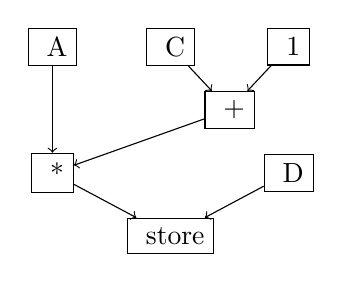
\begin{tikzpicture}[x=1.5cm, y=0.8cm]
                    \node[draw] (a) at (0, 0) {~A~};
                    \node[draw] (c) at (1, 0) {~C~};
                    \node[draw] (o) at (2, 0) {~1~};
                    \node[draw] (p) at (1.5, -1) {~+~};
                    \node[draw] (m) at (0, -2) {~*~};
                    \node[draw] (d) at (2, -2) {~D~};
                    \node[draw] (s) at (1, -3) {~store~};

                    \draw
                    (a) edge[->] (m)
                    (c) edge[->] (p)
                    (o) edge[->] (p)
                    (p) edge[->] (m)
                    (m) edge[->] (s)
                    (d) edge[->] (s);
                \end{tikzpicture}
            \end{center}
            \begin{itemize}
                \itemsep0em
                \item \textbf{register machine}
                    \begin{lstlisting}
                        load  r1 A
                        load  r2 C
                        add   r3 r2 #1 // r3 = C + 1
                        mul   r4 r1 r3 // r4 = r3 * A
                        store r4 D     // D = r4
                    \end{lstlisting}
                \item \textbf{stack machine}
                    \begin{lstlisting}
                        push  A        // load from A, push to stack
                        push  C
                        add   #1       // add 1 to the value on the top of stack
                        mul            // multiply the top two values on stack
                        store D        // store value on top of stack to memory
                    \end{lstlisting}
                    This can be difficult to trace.
                    It also has difficulty with copied operands (if an operand needs to be used twice).
                \item \textbf{dataflow machine}
                    \begin{lstlisting}
                        load  +3 A     // load from A, send to [mul]
                        load  +1 C     // load from C, send to [add] (next)
                        add   +1 #1    // add 1 to value received, send to [mul] (next)
                        mul   +1       // multiply values recieved, send to next
                        store D        // store value received
                    \end{lstlisting}
                    Recent dataflow instruction sets, such as \textit{EDGE}, \textit{TRIPS}, and \textit{Wavescalar}, bundle instructions into statically scheduled dataflow fragments.
                    Dynamically scheduling then occurs on the fragment level.
                \item \textbf{belt machine}
                    \begin{lstlisting}
                        load  A        // load A onto belt
                        load  C        // load C onto belt
                        add   -1 #1    // add 1 to the result of the previous instruction
                        mul   -1 -3    // multiply the results from positions -1 and -3 on the belt
                        store -1 D     // store the previous result to memory
                    \end{lstlisting}
                    The idea is that every instruction will write to a fresh register, with a finite (rolling) window of registers.
                    Operands are collected by an offset backwards to the instruction producing the operand.
                    There is very little energy consumption at the rename logic stage of the pipeline (almost none), compared to classical processors.
                    \medskip

                    The compiler needs to know the size of the belt.
                    For example, if we know an instruction will need something that will fall off the belt, it can be moved to the front of the belt.
                    Another approach is to spill it.
                    \medskip

                    Branches can have issues with this (and the dataflow machine).
                    If two branches both generate a value, the compiler will need to think about what values will be used downstream and have an additional copy instruction that moves it to a known location (forces the value to be completed).
            \end{itemize}
            The lecture then discusses examples of indirect jumps with a ~switch~.
        \subsection*{Chapter 4}
            The objective is to reduce the average memory access time, which is equal to $\text{HitTime} + \text{MissRate} \times \text{MissPenalty}$.
            This can be improved in three ways;
            \begin{enumerate}[1.]
                \itemsep0em
                \item reduce miss rate (hardware or software)
                \item reduce miss penalty
                \item reduce the time to hit in the cache
            \end{enumerate}
            \subsubsection*{Cache Miss Rate Reduction in Hardware}
                Misses can be classified into one of four classes (the last one isn't always included);
                \begin{itemize}
                    \itemsep0em
                    \item \textbf{compulsory} - experienced the first time the data has been seen in the machine (thought of as misses in an infinite cache)
                    \item \textbf{capacity} - cache cannot contain all the blocks needed (thought of as misses in any cache of that given capacity, misses in a fully associative cache)
                    \item \textbf{conflict} - caused by a compromise to the associativity of the cache
                    \item \textbf{coherence} - other processor / device has invalidated the data
                \end{itemize}
                When the cache size is small, the proportion of miss rates is dominated by capacity misses, however as it gets larger, compulsory misses and conflicts take up a larger proportion.
                Note that CPU benchmarks can often have low compulsory misses as they load some data and perform calculations on it.
                \medskip

                The lecture goes into the CPU benchmark suite by SPEC.
                Note that the main difference between integer and floating point benchmarks is not the type of arithmetic they perform.
                The former tends to intensively use pointers and hard-to-predict branches - they are difficult to parallelise either manually or by an automatic compiler.
                On the other hand, the latter tends to be more structured (control flow), operate on regular array data (rather than complex data structures), and benefit more from automatic parallelisation.
                There are also two types of benchmarks, speed (where we look at the execution time for one run), and rate (where we look at the maximum throughput, for example with a multicore machine).
                The SPEC benchmarks use the geometric mean of speedups (ratios) relative to the baseline.
                \medskip

                Comparing two different processors in the benchmarks show that architectural techniques benefits some workloads more than others - we should consider what the code is doing in the context of the architectural techniques in use.
                \medskip

                Consider the first 3 miss classes, assuming the total cache size isn't changed, and what happens if each of the following is changed;
                \begin{enumerate}[1.]
                    \itemsep0em
                    \item \textbf{block size}
                        \smallskip

                        Recall that the cache block / line is a unit of allocation, the tag is a memory address of a cached block, a set is a set of cache blocks indexed by a cache index, and a way is a set of alternative locations for a stored block in a given set.
                        There are also comparators and selectors, with the former verifying the tag matches an address, and the selector picking the data from the way that has the matching tag.
                        We use the index to select a set and then use the comparator to check each way for a hit.
                        \medskip

                        For a random benchmark, consider a (fixed) cache capacity of 16KB.
                        On the graph, there's a minimum miss rate at a block size of 64B; after which point as the block size increases, the miss rate increases.
                        Consider the extreme case, of a 1KB capacity and 256B block size.
                        In this scenario, we only have 4 distinct regions, and if the program accesses more than that, we will end up with misses.
                        The problem with very large cache lines is that we may speculatively fetch data into the large line and never use it (poor utilisation).
                        \medskip

                        Note that the graph in the slides also doesn't include the time; a larger block will take longer to load (assuming the bus width isn't changed) - this leads to a higher miss penalty.
                    \item \textbf{associativity}
                        \smallskip

                        A set-associative cache has more complex circuitry than a direct mapped cache (there's a MUX in the former).
                        While we may run into associativity conflicts, it may still have a faster speed due to the simple circuitry.
                        We assume that the cycle time gets worse as associativity increases; the miss rate is improved by increasing associativity, but the cache hit time is also increased slightly.
                        This could be improved with way-prediction (similar to squashing the hit in a direct-mapped cache).
                        \medskip

                        We ideally want the access time for a direct mapped cache and the miss rate of an associative cache.
                        An approach to doing this is to have two caches; one that's large and direct-mapped and another that's very small but fully associative.
                        Both caches are accessed in parallel.
                        When we index the direct mapped cache, we check if we have a hit - if it misses, we check the victim cache.
                        When we allocate into direct mapped cache, we displace the entry (if any) into the victim cache (recall the displacement causes the associativity conflicts).
                        On a victim cache hit, the data is allocated back into the direct-mapped cache.
                        \medskip

                        This is a competitive algorithm.
                        Given two strategies, each good for some but poor for others (direct-mapped and fully-associative).
                        We want to combine the two to create a composite strategy which cover each other, so we never suffer the worst case behaviour.
                        Consider the ski rental problem.
                        \medskip

                        In a skewed-associative cache, we use different indices in each cache way (for example a simple hash function, such as ~XOR~ some index bits with the tag bits and reorder index bits).
                        This is in contrast to the set-associative cache where the same index is used.
                        Consider a 2-way cache with three addresses, for the first function there's a chance that they may still conflict, but it's unlikely that the second hash function will cause another conflict (hence $f_0(~A~) = f_0(~B~) = f_0(~C~)$ but $f_1(~A~) \neq f_1(~B~) \neq f_1(~C~)$).
                        \medskip

                        The same idea is present for arrays; if we are really unlikely and get $f_0(~A[i]~) = f_0(~B[i]~) = f_0(~C[i]~)$ and $f_1(~A[i]~) = f_1(~B[i]~) = f_1(~C[i]~)$, it's very unlikely we end up with $f_0(~A[i + 1]~) = f_0(~B[i + 1]~) = f_0(~C[i + 1]~)$ and $f_1(~A[i + 1]~) = f_1(~B[i + 1]~) = f_1(~C[i + 1]~)$ (since the hash functions are pseudo-random).
                        In accessing arrays, if the addresses are exactly far enough apart, it could be in the case where all accesses conflict (worst case scenario) - the skewed-associative cache gets around this.
                        \medskip

                        The paper on the statistical model of this concludes that we get the miss rate of a more associative cache with fewer ways.
                        This also gives us more predictable average performance.
                        However, it requires a decoder per way, some latency is added for the hash function, and LRU is harder to implement.
                    \item \textbf{compiler}
                \end{enumerate}
                Misses can also be reduced in hardware by performing prefetching.
                After a cache miss, the stream buffer initiates a fetch for th next block (not allocated in the cache).
                On an access, the stream buffer is checked in parallel with the cache.
                The stream buffer is a FIFO queue.
                Similar idea to a victim cache.
                Modern processors do a similar technique, but allocate into the cache - with more associativity, cache `pollution' is less of a concern.
                \medskip

                This idea could be extended to track multiple access streams (one stream is good for instruction misses, multiple streams can be important for data, such as multiple arrays).
                \medskip

                Decoupled access-execute uses the idea that most programs have almost no dependence between floating point calculations and the sequence of addresses issued into the memory system.
                The address calculation issue instructions can be separated from the floating point arithmetic instructions that operate on the fetched data.
                As such, there are two processors, one for access and another for execute.
                The address-generation side can run ahead of the execution, allowing for values to be streamed into the execute processor (exploiting memory parallelism / pipelines).
                Loss of decoupling events can occur when the control flow depends on the execution results.
            \subsubsection*{Cache Miss Rate Reduction in Software}
                The prefetching mentioned in the previous lecture could be left entirely to the programmer and the compiler; many processors have software prefetch instructions.
                However, since hardware prefetching is generally quite good, there is significant overhead that may outweigh the benefit (slowing down the overall process) - it may be useful for simpler processors.
                The MIPS ~memcpy~ library code also prefetches the destination as every store implicitly has a cache load (hence both the source and destination need to be prefetched).
                \medskip

                If the prefetch would've generated a fault (accessing something illegal), we don't want the prefetch to fail but we also don't want the prefetch to fail either (it should be silently squashed).
                \medskip

                Instruction caches are also quite important, but are left out by benchmark suites as they tend to be quite small.
                \textit{McFarling} reduced instruction cache misses by choosing an instruction memory layout based on the call graph.
                Procedures are reordered in memory to reduce conflict misses.
                \medskip

                Data optimisations can also take place;
                \begin{itemize}
                    \itemsep0em
                    \item \textbf{storage layout transformations} \hfill spatial locality
                        \smallskip

                        Don't change the code, just how the variables are declared and the addresses in which they are stored.
                        \medskip

                        An example of this is array merging; an array of structs versus a struct of arrays.
                        \begin{lstlisting}
                            // before (2 sequential arrays)
                            int val[SIZE];
                            int key[SIZE];

                            // after (1 array of structs)
                            struct merge {
                              int val;
                              int key;
                            };
                            struct merge merged_array[SIZE];
                        \end{lstlisting}
                        The spatial locality can be improved, depending on the use case.
                        A counter-example is if we were to traverse the ~key~ array and get the ~value~ out, then the former should be stored contiguously.
                        However, if this is being used as a hash table for example, it would beneficial for the key and the value to reside in the same cache line (more likely with the array of structs).
                        \medskip

                        Row-major mapping maps indices horizontally, and similar for column-major (but vertically).
                        The Morton / quadtree layout gives spatial locality in two dimensions, giving a compromise between the two previous layouts.
                        A variant of this is used for texture caching by some GPUs.
                    \item \textbf{iteration space transformations} \hfill can also improve temporal locality
                        \smallskip

                        Change the order in which loops are executed.
                        \medskip

                        An example of this is loop fusion;
                        \begin{lstlisting}
                            // before
                            for (i = 0; i < N; i = i+1) {
                              for (j = 0; j < N; j = j+1) {
                                a[i][j] = 1 / b[i][j] * c[i][j]
                              }
                            }
                            for (i = 0; i < N; i = i+1) {
                              for (j = 0; j < N; j = j+1) {
                                d[i][j] = a[i][j] + c[i][j]
                              }
                            }

                            // after fusion
                            for (i = 0; i < N; i = i+1) {
                              for (j = 0; j < N; j = j+1) {
                                a[i][j] = 1 / b[i][j] * c[i][j]
                                d[i][j] = a[i][j] + c[i][j]
                              }
                            }

                            // after array contraction
                            for (i = 0; i < N; i = i+1) {
                              for (j = 0; j < N; j = j+1) {
                                cv = c[i][j]
                                a = 1 / b[i][j] * cv
                                d[i][j] = a + cv
                              }
                            }
                        \end{lstlisting}
                        After fusion, it should be faster due to less loop overhead, but also we avoid loading ~a~ from memory, as well as reloading ~c~.
                        The second transformation is safe if we don't need the array ~a~ after the loops have been executed; values can be transferred in scalar values rather than an array (contraction).
                        However, this (fusion) isn't always simple - for example a one-dimensional convolution / stencil (dependencies don't align nicely);
                        \begin{lstlisting}
                            // before
                            for (i = 1; i < N; i++) {
                              V[i] = (U[i - 1] + U[i + 1]) / 2
                            }
                            for (i = 1; i < N; i++) {
                              W[i] = (V[i - 1] + V[i + 1]) / 2
                            }

                            // after
                            V[1] = (U[0] + U[2]) / 2
                            for (i = 2; i < N; i++) {
                              V[i] = (U[i - 1] + U[i + 1]) / 2
                              W[i - 1] = (V[i - 2] + V[i]) / 2
                            }
                            W[N - 1] = (V[N - 2] + V[N]) / 2

                            // contraction is harder, need last two Vs (3 locations, use 4)
                            V[1] = (U[0] + U[2]) / 2
                            for (i = 2; i < N; i++) {
                              V[i % 4] = (U[i - 1] + U[i + 1]) / 2
                              W[i - 1] = (V[(i - 2) % 4] + V[i % 4]) / 2
                            }
                            W[N - 1] = (V[(N - 2) % 4] + V[N % 4]) / 2
                        \end{lstlisting}
                        This can be made fusable by shifting; the middle part of the loop is fusable, but there's some edges to manually perform.
                \end{itemize}
            \subsubsection*{Miss Penalty Reduction}
                A write-through policy involves writing to underlying layers; cached data can therefore always be discarded and the control bit only includes a valid bit.
                On the other hand, a write-back policy only updates the cache; cached data may have to be written back if discarded and control bits include both the valid bit as well as a dirty bit.
                The former has the advantage that the memory has the latest data (note that processors may have their own cache) and is simpler.
                On the other hand, the latter has lower requirements on the write bandwidth as the data is often overwritten multiple times - it also has better tolerance for slower memory.
                \medskip

                There are also policies in place for the case where it's a write-miss.
                Write allocate allocates a new cache line on a miss, whereas write non-allocate / write-around simply writes the data to the underlying layers (no new cache line is allocated).
                The former might make more sense for spatial locality, as something that's written could be read again soon.
                \medskip

                Consider a write buffer, sitting between the cache and lower memory.
                The purpose of the buffer is that we don't need to wait for the slower memory to write the data - however, this introduces yet another potential copy of this data.
                This applies regardless of write-back or write-through.
                Consider a program that's writing to a vector; ideally it's merged into a single entry in the buffer and written to the next level of the memory hierarchy only once.
                \medskip

                Typically on a miss, the entire cache block isn't loaded in parallel but rather word-by-word.
                Consider the case where the requested word is the first word in the block; ideally the processor can continue as soon as the requested word arrives (early restart).
                A more general / powerful idea is to have the critical word first; request the required word from the next level of the memory hierarchy first and then continue to populate the rest of the block.
                This is only really worthwhile in large blocks.
                \medskip

                This can also cause issues; especially in the case where the processor restarts and the next instruction also loads into another word in the \textbf{same} cache line.
                Each sector (or word) needs a validity bit; the cache block is the unit of allocation and deliver / transfer data in sectors.
                This validity bit tells us whether the sector has been updated already.
                \medskip

                Another strategy is to have a non-blocking / lockup-free cache.
                This allows the cache to continue to supply hits during a miss - it requires full / empty bits on registers or out-of-order execution and multi-bank memories.
                The idea of hit under miss reduces the miss penalty but allowing work to continue during while a miss is being handled.
                Hit under multiple miss or miss under miss lowers the effective miss penalty further my overlapping multiple misses.
                \medskip

                For an in-order pipeline, there are two options on a cache miss.
                The first is to freeze the pipeline in the memory access stage, stalling any other subsequent instructions.
                The miss status / handler registers (MSHR) keeps track of outstanding memory accesses and the registers waiting for these results, and only stalls the pipeline when an instruction references something that's needed.
                This provides some limited out-of-order execution (for loads).
                \medskip

                Hit under miss creates the opportunity for load instructions to execute out-of-order.
                From the thread running on the CPU, care will be taken to ensure the results from the load are the most recent data for that location written by this thread.
                However, in a multicore system, or a system with a DMA / memory mapped IO device, care should be taken knowing that load instructions can be reordered by this mechanism.
                Special instructions to be used to enforce the relative ordering of memory accesses, if we care.
                \medskip

                Another approach would be to add a second level cache.
                Let AMAT be the average memory access time, HT be the hit time, MR be the miss rate, and MP be the miss penalty;
                \begin{align*}
                    \text{MP}_\text{L1} & = \text{HT}_\text{L2} + \text{MR}_\text{L2} \times \text{MP}_\text{L2} \\
                    \text{AMAT} & = \text{HT}_\text{L1} + \text{MR}_\text{L1} \times \text{MP}_\text{L1} \\
                    & = \text{HT}_\text{L1} + \text{MR}_\text{L1} \times (\text{HT}_\text{L2} + \text{MR}_\text{L2} \times \text{MP}_\text{L2})
                \end{align*}
                The local miss rate is the misses in the cache divided by the total memory access to a given cache.
                On the other hand, the global miss rate is the misses in this cache divided by the total memory accesses from the CPU (this is what matters).
                \medskip

                The lecture continues for a bit discussing \textit{Haswell}'s cache hierarchy.
                \medskip

                Multi-level inclusion states that the $\text{L}_{n + 1}$ cache contains everything in $\text{L}_n$.
                We may sometimes allocate into L1 but not L2, or the other way around.
                We may also allocate into both L1 and L2, but not LLC.
                LLC (or L3) is sometimes used as a victim cache, once data is displaced from L2.
                If we don't assume multi-level inclusion, it's perfectly valid for L2 to displace something that's frequently being accessed in L1, as it sees no hits for that particular line.
                However, if we do rely on inclusion, then we need to track which lines cannot be displaced.
                \medskip

                Cache coherency is another argument for MLI; consider two cores each with its own L1 and L2 cache.
                Suppose the first core writes to an address that may be held in one of the caches of the second core.
                The second core needs to monitor all the bus traffic (loads, stores, accesses) of the other processor - if it sees an invalidation of a particular address, the second core's cache controller needs to check whether it has a cache copy of that address; if it does, then it needs to be invalidated.
                However, the L1 cache is typically very busy with processor traffic and shouldn't be touched.
                By relying on MLI, the L2 cache can be used to filter those invalidations.
            \subsubsection*{Hit Time Reduction and Address Translation}
                Consider the 8 stage pipeline in the \textit{MIPS R4000} (extended from the 5 stage pipeline of the \textit{MIPS R3000});
                \begin{itemize}
                    \itemsep0em
                    \item \textbf{IF} - first half of instruction fetch, PC selection happens here, also initiation of instruction cache access
                    \item \violet{\textbf{IS}} - second half of access
                    \item \textbf{RF} - instruction decode, register fetch, hazard checking, and instruction cache hit detection
                    \item \textbf{EX} - execution (effective address calculation, ALU operation, and branch target computation and condition evaluation)
                    \item \textbf{DF} - data fetch (first half of access to data cache)
                    \item \violet{\textbf{DS}} - second half of access
                    \item \violet{\textbf{TC}} - tag check, determine whether the data cache access was a hit
                    \item \textbf{WB} - write back for loads / register-register operations
                \end{itemize}
                Higher clock rate required deepening the pipelining, by splitting the fetch stages into two clock cycles (pipelining the cache itself).
                The DS stage could forward the instruction to a succeeding instruction, before the check is complete.
                If the check fails, then an additional cycle penalty is introduced.
                \medskip

                Consider the case where the first instruction is a load and the fourth instruction is an arithmetic operation that uses the result.
                The result can be passed into the execute stage of the fourth instruction before the tag check is complete.
                By designing a deeper pipeline, the clock cycle can be increased, but can potentially result in two stalls (e.g. if the instruction using the result was right after, whereas the 5 stage pipeline only had a single stall cycle).
                Similarly, this happens with the branch latency, if the conditions are evaluated during the EX phase.
                \medskip

                With the \textit{R4000}, stalls caused by waiting for results from FP units / access to FP hardware, account for a large amount of the lost performance, especially for floating point workloads.
                The next architecture from MIPS was an out-of-order processor.
                \medskip

                Currently, we're discussing reducing the hit time by pipelining, but it doesn't reduce the access latency (only throughput).
                With dynamic scheduling, this can still help.
                However, a bottleneck may arise from the bandwidth of the cache, especially in a processor that issues multiple instructions per cycle.
                A number of things can be done to support parallel access to the cache;
                \begin{itemize}
                    \itemsep0em
                    \item divide cache into several banks
                        \smallskip

                        Consider how each address can be mapped to a bank (low order bits of the cache index, etc.).
                        For example, a bank for even or odd addresses.
                        If addresses fall into odd/even pairs, then those accesses can be overlapped.
                    \item duplicate the cache
                        \smallskip

                        Stores are copied into both duplicates, but loads can be sent to whichever cache is idle.
                    \item multi-ported RAM (support two reads to different addresses very cycle)
                        \smallskip

                        A RAM array has a wordline per row, and a bitline per column.
                        In a multi-ported design, there would be multiple wordlines per row and multiple bitlines per column - allowing different rows and different columns to be activated simultaneously.
                \end{itemize}
                Simple processors can access memory directly (also what we've assumed so far) - the addresses are generated by the processor and directly used to access memory.
                However, we may want to run code in an isolated environment, preventing a crash in the code from bringing down the entire system, or preventing malicious code from having full access.
                Another use is to allow more than one application to be run at a time, preventing interference with each other, or even knowing about each other (each occupying a separate virtual machine).
                A major use is to use more memory than DRAM (for example, extending the memory hierarchy to HDD).
                Virtualising the memory can be done by adding address translation.
                \medskip

                Some approaches of this are as follows (note that the translation is done at ~TB~);
                \begin{itemize}
                    \itemsep0em
                    \item \textbf{physically-indexed, physically-tagged}
                        \begin{center}
                            \vspace{-\baselineskip}
                            \begin{minipage}[t]{0.33\textwidth}
                                \vspace{0pt}
                                \centering
                                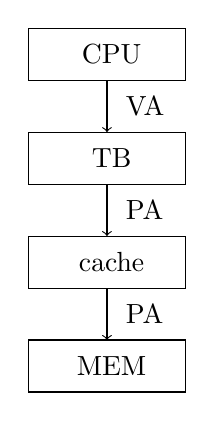
\begin{tikzpicture}[y=0.66cm]
                                    \begin{scope}[shift={(0, 0)}]
                                        \node at (1, -0.5) {~CPU~};
                                        \draw (0, 0) -- (2, 0) -- (2, -1) -- (0, -1) -- cycle;
                                    \end{scope}
                                    \begin{scope}[shift={(0, -2)}]
                                        \node at (1, -0.5) {~TB~};
                                        \draw (0, 0) -- (2, 0) -- (2, -1) -- (0, -1) -- cycle;
                                    \end{scope}
                                    \begin{scope}[shift={(0, -4)}]
                                        \node at (1, -0.5) {~cache~};
                                        \draw (0, 0) -- (2, 0) -- (2, -1) -- (0, -1) -- cycle;
                                    \end{scope}
                                    \begin{scope}[shift={(0, -6)}]
                                        \node at (1, -0.5) {~MEM~};
                                        \draw (0, 0) -- (2, 0) -- (2, -1) -- (0, -1) -- cycle;
                                    \end{scope}
                                    \draw
                                    (1, -1) edge[->, right] node{~VA~} (1, -2)
                                    (1, -3) edge[->, right] node{~PA~} (1, -4)
                                    (1, -5) edge[->, right] node{~PA~} (1, -6);
                                \end{tikzpicture}
                            \end{minipage}
                            \hfill
                            \begin{minipage}[t]{0.6\textwidth}
                                \vspace{0pt}
                                The processor operates on virtual addresses in its protected virtual environment.
                                After translation, we get physical addresses to access main memory.
                                The entire memory hierarchy operates on physical addresses after translation.
                            \end{minipage}
                        \end{center}
                    \item \textbf{virtually-indexed, virtually-tagged}
                        \begin{center}
                            \vspace{-\baselineskip}
                            \begin{minipage}[t]{0.33\textwidth}
                                \vspace{0pt}
                                \centering
                                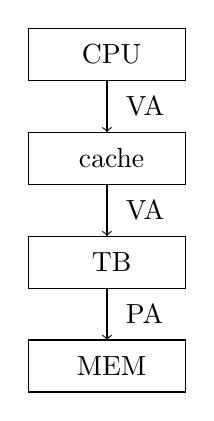
\begin{tikzpicture}[y=0.66cm]
                                    \begin{scope}[shift={(0, 0)}]
                                        \node at (1, -0.5) {~CPU~};
                                        \draw (0, 0) -- (2, 0) -- (2, -1) -- (0, -1) -- cycle;
                                    \end{scope}
                                    \begin{scope}[shift={(0, -2)}]
                                        \node at (1, -0.5) {~cache~};
                                        \draw (0, 0) -- (2, 0) -- (2, -1) -- (0, -1) -- cycle;
                                    \end{scope}
                                    \begin{scope}[shift={(0, -4)}]
                                        \node at (1, -0.5) {~TB~};
                                        \draw (0, 0) -- (2, 0) -- (2, -1) -- (0, -1) -- cycle;
                                    \end{scope}
                                    \begin{scope}[shift={(0, -6)}]
                                        \node at (1, -0.5) {~MEM~};
                                        \draw (0, 0) -- (2, 0) -- (2, -1) -- (0, -1) -- cycle;
                                    \end{scope}
                                    \draw
                                    (1, -1) edge[->, right] node{~VA~} (1, -2)
                                    (1, -3) edge[->, right] node{~VA~} (1, -4)
                                    (1, -5) edge[->, right] node{~PA~} (1, -6);
                                \end{tikzpicture}
                            \end{minipage}
                            \hfill
                            \begin{minipage}[t]{0.6\textwidth}
                                \vspace{0pt}
                                Here, we only do a memory access on a cache miss.
                                As such, the cache ins virtually indexed.
                                On a cache miss, the addresses is then translated to access main memory.
                                The advantage is that it has a better hit time, as it doesn't always have to go through translation (we can get an L1 cache hit without translation).
                                This can run into issues when the processes switch (cache contains data from process being interrupted) - causes correctness (synonym / homonym) problems.
                            \end{minipage}
                        \end{center}
                    \item \textbf{virtually-indexed, physically-tagged}
                        \begin{center}
                            \vspace{-\baselineskip}
                            \begin{minipage}[t]{0.33\textwidth}
                                \vspace{0pt}
                                \centering
                                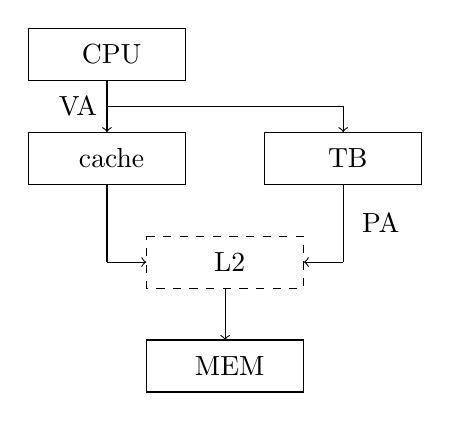
\begin{tikzpicture}[y=0.66cm]
                                    \begin{scope}[shift={(0, 0)}]
                                        \node at (1, -0.5) {~CPU~};
                                        \draw (0, 0) -- (2, 0) -- (2, -1) -- (0, -1) -- cycle;
                                    \end{scope}
                                    \begin{scope}[shift={(0, -2)}]
                                        \node at (1, -0.5) {~cache~};
                                        \draw (0, 0) -- (2, 0) -- (2, -1) -- (0, -1) -- cycle;
                                    \end{scope}
                                    \begin{scope}[shift={(3, -2)}]
                                        \node at (1, -0.5) {~TB~};
                                        \draw (0, 0) -- (2, 0) -- (2, -1) -- (0, -1) -- cycle;
                                    \end{scope}
                                    \begin{scope}[shift={(1.5, -4)}]
                                        \node at (1, -0.5) {~L2~};
                                        \draw[dashed] (0, 0) -- (2, 0) -- (2, -1) -- (0, -1) -- cycle;
                                    \end{scope}
                                    \begin{scope}[shift={(1.5, -6)}]
                                        \node at (1, -0.5) {~MEM~};
                                        \draw (0, 0) -- (2, 0) -- (2, -1) -- (0, -1) -- cycle;
                                    \end{scope}
                                    \draw
                                    (1, -1) edge[->, left] node{~VA~} (1, -2)
                                    (1, -1.5) -- (4, -1.5) edge[->] (4, -2)
                                    (4, -3) edge[right] node{~PA~} (4, -4.5)
                                    (4, -4.5) edge[->] (3.5, -4.5)
                                    (1, -3) -- (1, -4.5) edge[->] (1.5, -4.5)
                                    (2.5, -5) edge[->] (2.5, -6);
                                \end{tikzpicture}
                            \end{minipage}
                            \hfill
                            \begin{minipage}[t]{0.6\textwidth}
                                \vspace{0pt}
                                We want the hit time performance of VIVT with the semantic cleanliness of PIPT.
                                The key idea is that the translation is done in parallel with the L1 cache access.
                                The L1 cache accesses uses the low order bits to generate data as well as a tag.
                                Meanwhile, the translation translates the page number part of the address, and produces a physical translation of the page number.
                                The physical address can be compared with the tag.
                                If we have a hit, we have a low latency hit, otherwise, on a miss we have a physical address to access the L2 cache.
                            \end{minipage}
                        \end{center}
                \end{itemize}
                The original motivation for address translation was virtual memory - creating a virtual address space for a process, larger than the physical memory.
                Translations map virtual addresses either to physical pages in the RAM of the machine, or inactive pages stored on the swapping disk.
                Ideally, the process runs quickly the majority of the time reading from RAM, but may require a page that is inactive, causing a fault and raising an interrupt.
                The OS then deals with it and hopefully finds the data on the drive, and allocates it to a vacant page in the memory (otherwise fail).
                The allocation to a page in memory corrects the mapping.
                \medskip

                The processor produces a virtual address, that consists of the page number ~P~ and ~W~ (word number) - an offset in that page.
                Note that ~B~ denotes the page frame address.
                The processor also has a pointer to the \textbf{current page table} (process page table), which contains a mapping from page numbers to physical locations (long with some metadata).
                \medskip

                This can be sped up by adding caches (including caching the address translation).
                This is done with a TLB (translation lookaside buffer), containing recently accessed page table values; this table (also ~TB~ before) is typically highly associative and closely integrated with the L1 cache.
                \medskip

                We want one computer to be able to run two processes in isolation from each other, without knowing about each other.
                We don't want to care about what machine we have, nor do we care about what other processes are running.
                Each process has a virtual address space (begins at zero), which maps to different physical addresses.
                Another use case is that two processes may share the same code (such as shared libraries which are dynamically linked); but have different data.
                Ideally, we don't want the shared code (which is read-only) to be in different locations, but rather share the same physical location.
                \medskip

                When memory is allocated, the process asks the OS to allocate a virtual address space, which needs to be zeroed (cleared).
                The OS commonly allocates a single \textbf{shared} frame that is zeroed out, and points the virtual addresses to it.
                However, when the process begins to write, a fault occurs and a new frame is allocated, with the mapping fixed.
                Permissions need to be associated with these pages; a bit allowing writing and a bit to allow reading (hence all initial zeroed pages need to be read-only, after the mapping is updated, the bit is flipped).
                This trick is known as copy-on-write.
                \medskip

                Another use is to have two processes sharing the same memory-mapped file, with both processes having both read and write permissions.
                \medskip

                In address translation, there can be issues;
                \begin{itemize}
                    \itemsep0em
                    \item \textbf{homonyms} (same sound, different meaning)
                        \smallskip

                        Same virtual address pointing to two different physical addresses in different processes.
                        If we have a virtually-indexed cache, it must be flushed between context switches (expensive, especially for a large cache), or a process ID needs to be included in the cache tag.
                    \item \textbf{synonyms} (different sound, same meaning)
                        \smallskip

                        Different virtual addresses (different processes, or even the same process) pointing to the same physical address.
                        In a virtually-indexed cache, a virtual address could be cached multiple times under different physical addresses, and updates in one copy may not be reflected in the other.
                        A solution is to prevent synonyms from co-existing in the cache (if they are in the cache, then it must map to the same location); the OS could force synonyms to have the same index bits in a direct mapped cache (page colouring).
                \end{itemize}
                A 32-bit address consists of a 20-bit page number, followed by a 12-bit page offset (not translated).
                In the idea of a VIPT system, only the page offset (untranslated) is used to index the cache.
                In parallel, the page number is used to index the TLB, to obtain a translated page number (physical address).
                The translated physical address can be checked against the tag from the L1 cache - if these match, then we have a hit (low hit penalty).
                However, if it's a miss, we have a translated address that can be sent to the L2 cache.
                However, this limits the cache to the page size, since we can only use untranslated cache index bits - there are two options to use bigger caches;
                \begin{itemize}
                    \itemsep0em
                    \item \textbf{higher associativity}
                        \smallskip

                        Multiple ways could be indexed with the same bits (not requiring more bits), but having multiple ways gives us a bigger cache.
                        This is quite commonly done, and as a consequence, L1 data and instruction caches are often highly associative.
                        The associativity and the size matches can also be seen to match the aforementioned constraint.
                    \item \textbf{page colouring}
                        \smallskip

                        This requires the OS to help.
                        A (cache synonym) conflict occurs when two cache blocks have the same tag (physical address) are mapped to two different virtual addresses.
                        \medskip

                        Consider a 14-bit cache index, which is more bits than the 12-bit page offset (untranslated) from the virtual address.
                        The two bits are from the untranslated page number, which will then be translated.
                        As such, we need to ensure that when we choose how data is allocated into memory that we don't have the consistency problem as a result.
                        \medskip

                        A case for this is when two processes map the same file into memory; ideally we'd want their virtual address spaces to be the same.
                        This is a bigger constraint than required; we just need to ensure that the extra bits used match (if this is satisfied, we don't have the synonym conflict problem).
                        \medskip

                        The ~mmap~ system call in Linux has the operating system choose an implementation dependent mapping constraint.
                \end{itemize}
                Going back to the VIPT structure, the virtual addresses index the cache using the untranslated bits.
                Whether we get a conflict in the L1 cache is independent of any translations.
                However, associativity conflicts in the L2 cache depend on how the addresses are translated; they may be translated in such a way that means the cache index bits in the L2 cache are the same.
                This means that running the same program on the same data could lead to different associativity conflicts, due to different virtual-to-physical mappings.
                \medskip

                The OS typically has heuristics to avoid this - choosing non-conflicting pages for frequently-accessed data (page colouring for conflict avoidance).
                \medskip

                TLBs may need to support mappings for different size pages, for example the \textit{Haswell} TLB needs to support 128 mappings for 4KB pages and 8 2MB page mappings in the ITLB, as well as 64 mappings for 4KB pages, 8 2MB page mappings, and 4 mappings for 1GB pages in the DTLB.
            \subsubsection*{DRAM and Memory Parallelism}
                The DRAM device is a large array of cells holding data.
                DRAM emphasis capacity, leading us to have a single transistor design where data is stored on a capacitor.
                It's a two dimensional array, where horizontally we have wordlines and vertically we have bitlines.
                Data is stored as a charge on the capacitor - when we activate a wordline, an entire row of cells is activated, and charge flows along all of the bitlines.
                The row address goes into a DEMUX, which selects the row, and the charges flow into a sense amplifier (comparator), which goes into a latch for all the bits in an entire row.
                The column address bits go into a data selector (a MUX), which routes the data from the latch into the output.
                However, note that once the row is read, the data is lost from the capacitors.
                Once the data is latched, the switch is enabled on RAS and data is \textbf{written back} into the memory cell - the transistor is reactivated and the charge is allowed to flow in the opposite direction to recharge the capacitors.
                Data is written to RAM in the same way.
                \medskip

                However, the charge may leak out in a number of ways.
                As such, the DRAM needs to be refreshed (otherwise the charges may become indistinguishable).
                The data needs to be written back even when not accessing the rows with some refresh mechanism.
                As a consequence, DRAM is unavailable during refreshes, which happens every 64 milliseconds, or more frequently if the device is hot (self managed).
                This is typically managed by a microcontroller on the chip, and is typically done a few wordlines at a time in a cyclic fashion.
                This spreads out the interruption to general service over time.
                \medskip

                Once a row is selected, the entire row is latched, allowing elements in the row (different columns) to be accessed with lower latency.
                For example, with a 60ns ($t_\text{RAC}$) DRAM;
                \begin{itemize}
                    \itemsep0em
                    \item can only perform a row access every 110ns ($t_\text{RC}$)
                    \item perform column access in 15ns ($t_\text{CAC}$) but time between column access is at least 35ns ($t_\text{PC}$) - in practice, additional delays make it between 40ns and 50ns
                \end{itemize}
                The row access cycle time is longer than the row access time, as data needs to be written back after reading.
                \medskip

                The architecture of a SDRAM chip may have multiple banks of DRAM arrays, each with its own sense amplifier array and individual row access latch and decoders.
                This allows different rows from different banks to be accessed in parallel with one another.
                Each bank has its own read latch and column decoder, to select data and read it out.
                \medskip

                We want to run right up to the limit of reliability, to make the device as small as possible.
                As such, there's a risk that errors creep in, possibly even from interference from neighbouring cells, or radiation (high-energy cosmic rays, single-event upsets - an individual bit being flipped).
                The basic idea is to add redundancy through parity (for example, an even or odd number of 1s) / ECC bits.
                Parity doesn't allow for recovery.
                An example for a Hamming code is as follows; 64 data bits and 8 parity bits.
                Consider the data bits as forming a 64 element vector, each with one bit per element.
                Each individual potential 64 bit value occupies a point in 64-dimensional space.
                More dimensions are added into this space to separate the valid points.
                A SEU moves that vector from where it should be into an adjacent location in that space; we want to ensure that the adjacent locations don't correspond to a valid data value.
                A single error pushes us slightly away from a valid position, and can therefore be pushed back.
                Ideally, we want to be able to handle failures of entire chips; the idea of RAID with hard drives works here too.
                \medskip

                We can test DRAM by trying to cause memory upsets.
                Imagine an array, with one row that we care about, and two adjacent rows.
                A program could repeatedly write into the adjacent rows, trying to flip bits in the row we care about.
                As the row gets closer to the refresh deadline, it becomes more vulnerable to an upset.
                The \textit{Rowhammer} attack does this.
                This can be mitigated with ECC, or adaptive refresh which counts accesses and refreshes potential victim rows earlier.
                \medskip

                The lecture then goes into further topics in DRAM, including energy optimisations, on-memory processing, stacking, bulk copying and zeroing, and non-volatile memory.
                \medskip

                The simple organisation of main memory has the CPU, cache, bus, and memory all at the same widths.
                A wider organisation of main memory could have parallel data transfer, with the same address in all banks (with a wider bus).
                Another approach, an interleaved organisation, could allow multiple banks of memory to be addressed individually; parallel addressing as well as parallel data transfer.
                Consideration should be taken to spread accesses across the banks.
        \subsection*{November 2 - Live Lecture}
            The intuition for the skewed two-way set-associative cache is that there is no restriction on what the functions are, as long as they are different.
            However, it also needs more than just the low-order $k$ bits, to get more `randomness'.
            \medskip

            When executing a store, there is a chance the address is in the L1 cache.
            Consider the case where it isn't in the L1 cache.
            We can allocate in on a read but not a store (write non-allocate) - this may not be ideal as when we write into memory we tend to want to read it back, and the principals of locality tell us that we might want to do it soon.
            Consider a cache line, and storing only affecting a word at a time.
            A common access pattern is writing successive words; which would require multiple writes to L2 (for non-allocate).
            \medskip

            The stream buffer assumes a fully parallel lookup.
            \medskip

            We have several structures mechanisms that result in copies of data being in different places.
            We need to look at all these places in parallel;
            \begin{itemize}
                \itemsep0em
                \item L1D
                \item write buffer
                \item stream buffer (prefetching mechanism)
                \item victim cache
                \item store queue
            \end{itemize}
            All of these structures are similar and are tag / comparator lookup checks.
            The store queue should be checked first (not in parallel); we should check if the data we want is generated by an uncommitted (earlier) store instruction.
        \subsection*{Chapter 5}
            \subsubsection*{Microarchitectural Sidechannels - Spectre and Meltdown}
                %TODO https://imperial.cloud.panopto.eu/Panopto/Pages/Viewer.aspx?id=eb82fea9-6431-4ad8-95e6-add500114d40
\end{document}